\documentclass[a4paper]{article}

\setlength{\parindent}{0pt}
\setlength{\parskip}{1em}

\pagestyle{headings}

\usepackage{amssymb}
\usepackage{amsmath}
\usepackage{amsthm}
\usepackage{mathtools}
\usepackage{graphicx}
\usepackage{hyperref}
\usepackage{color}
\usepackage{microtype}
\usepackage{tikz}
\usepackage{pgfplots}
\usepackage{pgfplotstable}

\newcommand{\N}{\mathbb{N}}
\newcommand{\Q}{\mathbb{Q}}
\newcommand{\Z}{\mathbb{Z}}
\newcommand{\R}{\mathbb{R}}
\newcommand{\C}{\mathbb{C}}
\newcommand{\D}{\mathcal{D}}
\renewcommand{\S}{\mathcal{S}}
\renewcommand{\P}{\mathbb{P}}
\newcommand{\F}{\mathbb{F}}
\newcommand{\E}{\mathbb{E}}
\newcommand{\bra}{\langle}
\newcommand{\ket}{\rangle}


\graphicspath{{Image/}}

\hypersetup{
    colorlinks=true,
    linktoc=all,
    linkcolor=blue
}

\theoremstyle{definition}
\newtheorem*{axiom}{Axiom}
\newtheorem*{claim}{Claim}
\newtheorem*{conv}{Convention}
\newtheorem*{coro}{Corollary}
\newtheorem*{defi}{Definition}
\newtheorem*{eg}{Example}
\newtheorem*{lemma}{Lemma}
\newtheorem*{notation}{Notation}
\newtheorem*{prob}{Problem}
\newtheorem*{post}{Postulate}
\newtheorem*{prop}{Proposition}
\newtheorem*{rem}{Remark}
\newtheorem*{thm}{Theorem}

\DeclareMathOperator{\vdiv}{div}
\DeclareMathOperator{\grad}{grad}
\DeclareMathOperator{\curl}{curl}
\DeclareMathOperator{\Ann}{Ann}
\DeclareMathOperator{\Fit}{Fit}
\DeclareMathOperator{\Diag}{Diag}
\DeclareMathOperator{\tr}{tr}
\DeclareMathOperator{\im}{im}
\DeclareMathOperator{\Mat}{Mat}
\DeclareMathOperator{\Log}{Log}
\DeclareMathOperator{\Isom}{Isom}
\DeclareMathOperator{\Mesh}{Mesh}
\DeclareMathOperator{\Sym}{Sym}
\DeclareMathOperator{\Aut}{Aut}
\DeclareMathOperator{\cosech}{cosech}
\DeclareMathOperator{\Card}{Card}
\DeclareMathOperator{\Gal}{Gal}


\setcounter{section}{-1}

\begin{document}

\title{Representation Theory}

\maketitle

\newpage

\tableofcontents

\newpage

\section{Introduction}
Representaiton theory is the theory of how \emph{groups} act as groups of linear transformations on \emph{vector spaces}. 

Here the groups are either \emph{finite}, or \emph{compact topological groups} (infinite), for example, $SU(n)$ and $O(n)$. The vector spaces we conside are finite dimensional, and usually over $\C$. Actions are \emph{linear} (see below).

Some books: James-Liebeck (CUP); Alperin-Bell (Springer); Charles Thomas, \emph{Representations of finite and Lie groups}; Onlne notes: SM, Teleman; P.Webb \emph{A course in finite group representation theory} (CUP); Charlie Curtis, \emph{Pioneers of representation theory} (history).

\newpage

\section{Group actions}

Throughout this course, if not specified otherwise:\\
$\bullet$ $F$ is a field, usually $\C$, $\R$ or $\Q$. When the field is one of these, we are discussing \emph{ordinary representation theory}. Sometimes $F=F_p$ or $\bar{F}_p$ (algebraic closure, see Galois Theory), in which case the theory is called \emph{modular representation theory};\\
$\bullet$ $V$ is a vector space over $F$, always finite dimensional;\\
$GL(V) =\{\theta : V \to V, \theta$ linear, invertible$\}$, i.e. $\det \theta \neq 0$.

Recall from Linear Algebra:\\
If $\dim_F V = n < \infty$, choose basis $e_1,...,e_n$ over $F$, so we can identify it with $F^n$. Then $\theta \in GL(V)$ corresponds to an $n \times n$ matrix $A_\theta = (a_{ij})$, where $\theta(e_j) = \sum_i a_{ij} e_i$. In fact, we have $A_\theta \in GL_n(F)$, the general linear group.

(1.1) $GL(V) \cong GL_n(F)$ as groups by $\theta \to A_\theta$ ($A_{\theta_1 \theta_2} = A_{\theta_1} A_{\theta_2}$ and bijection).\\
Choosing different basis gives different isomorphism to $GL_n(F)$, but:

(1.2) Matrices $A_1,A_2$ represent the same element of $GL(V)$ w.r.t different bases iff they are conjugate (similar), i.e. $\exists X \in GL_n(F)$ s.t. $A_2 =XA_1 X^{-1}$.

Recall that $\tr(A) = \sum_i a_{ii}$ where $A = (a_{ij})$, the \emph{trace} of $A$.

(1.3) $\tr(XAX^{-1}) = \tr(A)$, hence we can define $\tr(\theta) = \tr(A_{\theta_1})$ independent of basis.

(1.4) Let $\alpha \in GL(V)$ where $V$ in f.d. over $\C$, with $\alpha^m = \iota$ for some $m$ (here $\iota$ is the identity map). Then $\alpha$ is diagonalisable.

Recall $EndV$ is the set of all ilnear maps $V \to V$, e.g. $End(F^n) =M_n(F)$ some $n \times n$ matrices.

(1.5) \emph{Proposition.} Take $V$ f.d. over $\C$, $\alpha \in End(V)$. Then $\alpha$ is diagonalisable iff there exists a polynomial $f$ with distinct linear factors with $f(\alpha) = 0$. For example, in (1.4), where $\alpha^m = \iota$, we take $f = X^m - 1 = \prod_{j=0}^{m-1} (X-\omega^j)$ where $\omega = e^{2\pi i/m}$ is the ($m^{th}$) root of unity. In fact we have:

(1.4)* A finite family of commuting separately diagonalisable automorphisms of a $\C$-vector space can be simultaneously diagonalised (useful in abelian groups).

Recall from Group Theory:\\
(1.6) The symmetric group, $S_n = Sym(X)$ on the set $X = \{1,...,n\}$ is the set of all permutations of $X$. $|S_n| = n!$. The alternating group $A_n$ on $X$ is the set of products of an even number of transpositions (2-cycles). $|A_n| = \frac{n!}{2}$.

(1.7) Cyclic groups of order $m$: $C_m = <x:x^m = 1>$. For example, $(\Z/m\Z, +)$; also, the group of $m^{th}$ roots of unity in $\C$ (inside $GL_1(\C)$ = $\C^*$, the multiplicative group of $\C$). We also have the group of rotations, centre $O$ of regular $m-$gon in $\R^2$ (inside $GL_2(\R)$).

(1.8) Dihedral groups $D_{2m}$ of order $2m = <x,y: x^m = y^2 = 1, yxy^{-1} = x^{-1}>$. Think of this as the set of rotations and reflections preserving a regular $m$-gon.

(1.9) Quaternion group, $Q_8 = <x,y|x^4 = 1, y^2 = x^2, yxy^{-1} = x^{-1}>$ of order $8$. For example, in $GL_2(\C)$, put $i={{i\ 0} \choose {0 \ i}}, j = {{0 \ 1} \choose {-1 \ 0}}, k = {{0 \ i} \choose {i \ 0}}$, then $Q_8 = \{\pm I_2, \pm i, \pm j, \pm k\}$.

(1.10) The conjugacy class (ccls) of $g \in G$ is $\mathcal{C}_G(g) = \{xgx^{-1} : x \in G\}$. Then $|\mathcal{C}_G (g) | = |G:C_G(g)|$, where $C_G(g) = \{x \in G : xg = gx\}$, the centraliser of $g \in G$.

(1.11) Let $G$ be a group, $X$ be a set. $G$ acts on $X$ if there exists a map $\cdot: G \times X \to X$ by $(g,x) \to g\cdot x$ for $g \in G$, $x \in X$, s.t. $1 \cdot x = x$ for all $x \in X$, $(gh) \cdot x = g \cdot (h\cdot x)$ for all $g,h \in G, x \in X$.

(1.12) Given an action of $G$ on $X$, we obtain a homomorphism $\theta: G \to Sym(X)$, called the \emph{permutation representation} of $G$.
\begin{proof}
For $g \in G$, the function $\theta_g: X \to X$ by $x \to gx$ is a permutation on $X$, with inverse $\theta_{g^{-1}}$. Moreover, $\forall g_1,g_2 \in G$, $\theta_{g_1 g_2} = \theta_{g_1} \theta_{g_2}$ since $(g_1g_2) x = g_1(g_2 x)$ for $x \in X$.
\end{proof}

\newpage

\section{Basic Definitions}
\subsection{Representations}

Let $G$ be finite, $F$ be a field, usually $\C$.
\begin{defi} (2.1)\\
Let $V$ be a f.d. vector space over $F$. A (linear, in some books) \emph{representation} of $G$ on $V$ is a group homomorphism 
\begin{equation*}
\begin{aligned}
\rho = \rho_V: & G &\to GL(V)
\end{aligned}
\end{equation*}
Write $\rho_g$ for the image $\rho_V(g)$; so for each $g \in G$, $\rho_g \in GL(V)$, and $\rho_{g_1 g_2} = \rho_{g_1} \rho_{g_2}$, and $(\rho_g)^{-1} = \rho_{g^{-1}}$.\\
The \emph{dimension} (or \emph{degree}) of $\rho$ is $\dim_F V$.
\end{defi}

(2.2) Recall $\ker \rho \triangleleft G$ (kernel is a normal subgroup), and $G/\ker \rho \cong \rho(G) \leq GL(V)$ (1st isomorphism theorem). We say $\rho$ is \emph{faithful} if $\ker \rho = 1$.

An alternative (and equivalent) approach is to observe that a representation of $G$ on $V$ is "the same as" a \emph{linear action} of $G$:

\begin{defi} (2.3)\\
$G$ \emph{acts linearly} on $V$ if there exists a \emph{linear action}
\begin{equation*}
\begin{aligned}
G \times V &\to V\\
(g,v) &\to gv
\end{aligned}
\end{equation*}
By linear action we mean: (action) $(g_1 g_2) v = g_1(g_2 v)$, $1v=v$ $\forall g_1,g_2 \in G, v \in V$, and (linear) $g(v_1+v_2) = gv_1+gv_2$, $g(\lambda v) = \lambda gv$ $\forall g \in G, v_1,v_2 \in V, \lambda \in F$.\\
Now if $G$ acts linearly on $V$, the map
\begin{equation*}
\begin{aligned}
G &\to GL(V)\\
g &\to \rho_g
\end{aligned}
\end{equation*}
with $\rho_g:v \to gv$ is a representation of $G$. Conversely, given a representation $\rho: G \to GL(V)$, we have a linear action of $G$ on $V$ via $g \cdot v := \rho(g) v$ $\forall v \in V, g \in G$.
\end{defi}

(2.4) In (2.3) we also say that $V$ is a $G$-space or that $V$ is a $G$-module. In fact if we define the \emph{group algebra} $FG$, or $F[G]$, to be $\{ \sum \alpha_j g: \alpha_j \in F\}$ with natural addition and multiplication, then $V$ is actually a $FG$-module (in the sense from GRM).

(2.5) $R$ is a \emph{matrix representation} of $G$ of degree $n$ if $R$ is a homomorphism $G \to GL_n (F)$. Given representation $\rho:G \to GL(V)$ with $\dim_F V=n$, fix basis $B$; we get matrix representation
\begin{equation*}
\begin{aligned}
G &\to GL_n(F)\\
g &\to [\rho(g)]_B
\end{aligned}
\end{equation*}
Conversely, given matrix representation $R:G \to GL_n(F)$, we get representation
\begin{equation*}
\begin{aligned}
\rho: G &\to GL(F^n)\\
g &\to \rho_g
\end{aligned}
\end{equation*}
via $\rho_g(v) = R_g v$ where $R_g$ is the matrix of $g$.

\begin{eg} (2.6)\\
Given any group $G$, take $V=F$ the 1-dimensional space, and 
\begin{equation*}
\begin{aligned}
\rho:G &\to GL(F)\\
g &\to (id: F \to F)
\end{aligned}
\end{equation*}
is known as the trivial representation of $G$. So $\deg \rho = 1$ ($\dim_F F = 1$).
\end{eg}

\begin{eg} (2.7)\\
Let $G=C_4 = <x:x^4=1>$. Let $n=2$, and $F=\C$. Note that any $R:x \to X$ will determine $x^j \to X^j$ as it is a homomorphism, and also we need $X^4 = I$. So we can take $X$ to be diagonal matrix -- any such with diagonal entries a root to $x^4=1$, i.e. $\{\pm 1,\pm i\}$, or if $X$ is not diagonal then it will be similar to a diagonal matrix by (1.4) ($X^4=I$).
\end{eg}

\subsection{Equivalent representations}

\begin{defi} (2.8)\\
Fix $G,F$. Let $V,V'$ be $F$-spaces, and $\rho:G \to GL(V)$, $\rho': G \to GL(V')$ which are representations of $G$. The linear map $\phi: V \to V'$ is a $G$-homomorphism if $$\phi\rho(g) = \rho'(g)\phi \forall g \in G (*)$$ We can understand this more by the following diagram:

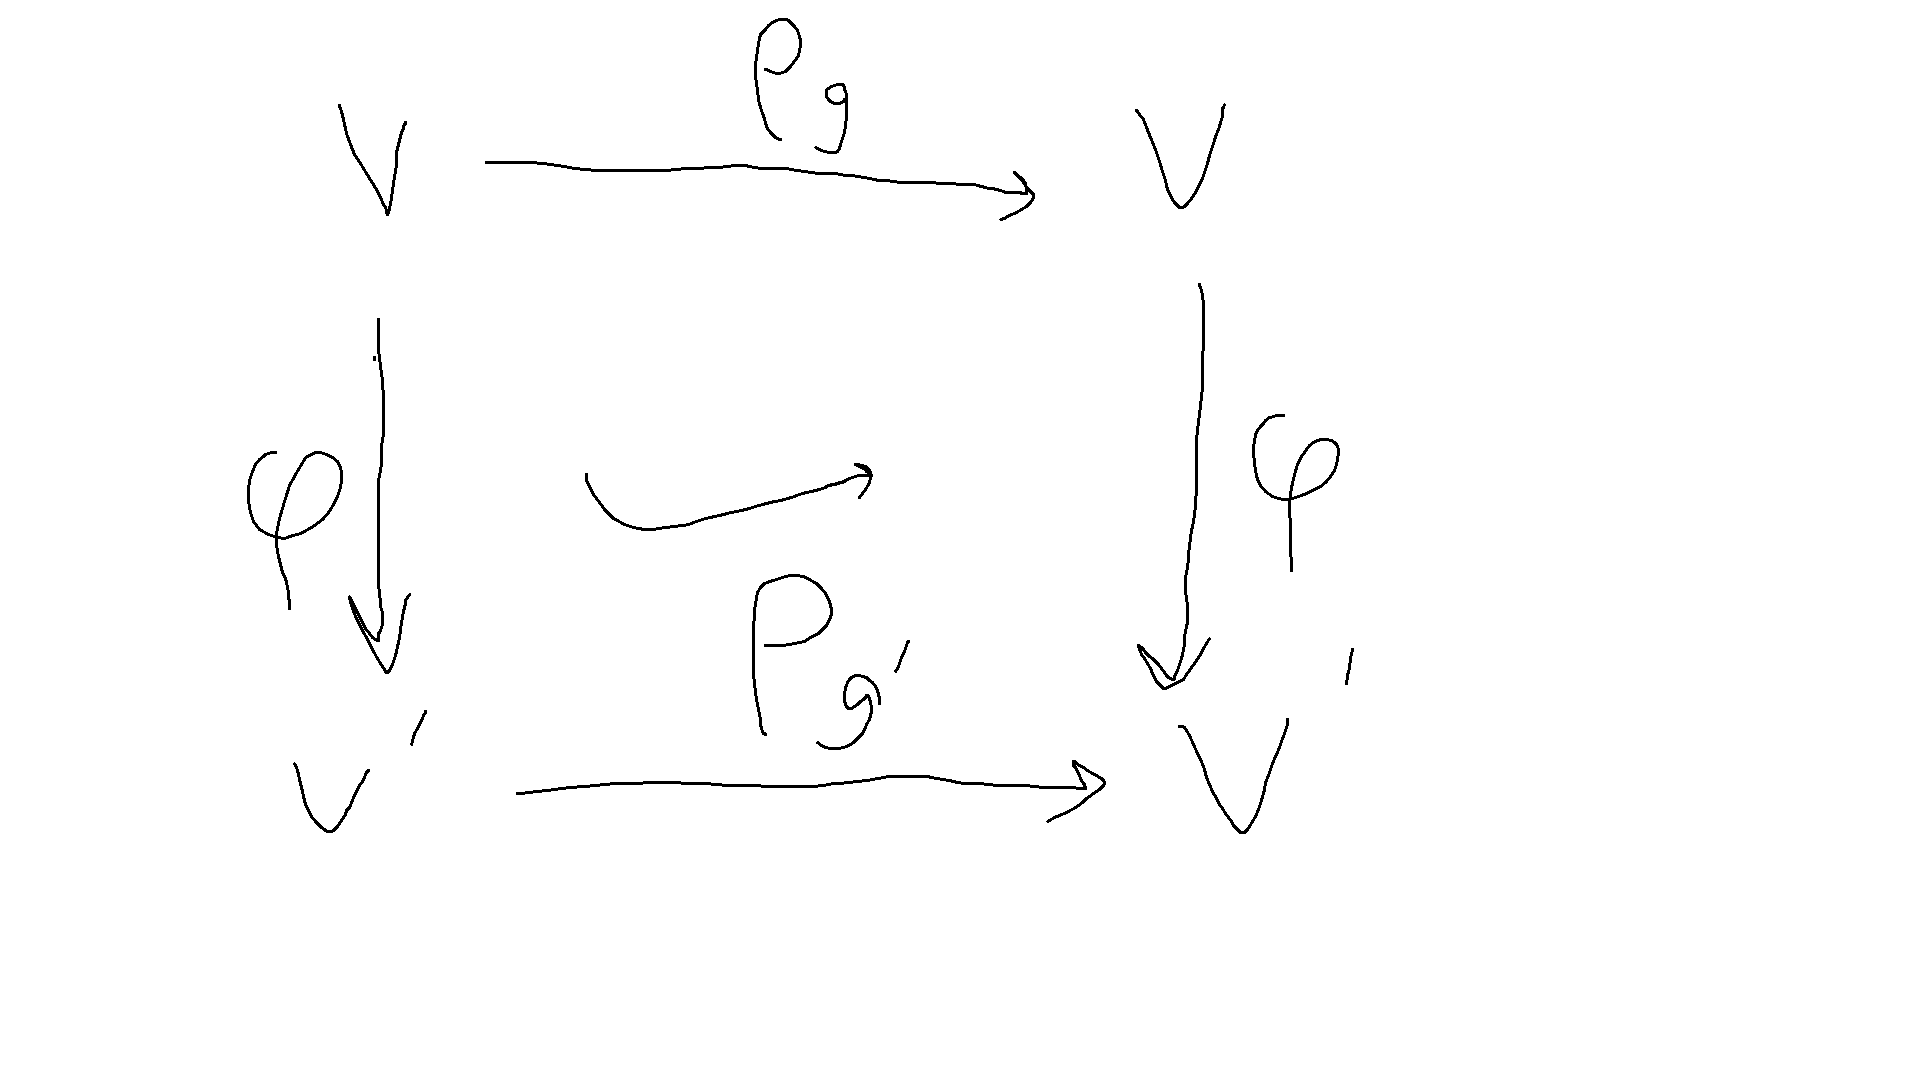
\includegraphics[scale=0.5]{image/Rep_01.png}

We say $\phi$ \emph{intertwines} $\rho,\rho'$. Write $Hom_G(V,V')$ for the $F$-space of all these.\\
$\phi$ is a $G$-isomorphism if it is also bijective; if such $\phi$ exists, $\rho,\rho'$ are isomorphic/equivalent representations. If $\phi$ is a $G$-isomorphism, we can write $(*)$ as $\rho' = \phi\rho\phi^{-1}$.
\end{defi}

\begin{lemma} (2.9)\\
The relation "being isomorphic" is an equivalent relation on the set of all representations of $G$ (over $F$).
\end{lemma}

\begin{rem} (2.10)\\
If $\rho,\rho'$ are isomorphic representations, they have the same dimension.

The converse may be false: $C_4$ has four non-isomorphic 1-dimensional representations: if $\omega = e^{2\pi i/4}$ then they are $\rho_j(x^i) = \omega^{ij}$ ($0 \leq i \leq 3$).
\end{rem}

\begin{rem} (2.11)\\
Given $G$, $V$ over $F$ of dimension $n$ and $\rho:G \to GL(V)$. Fix basis $B$ for $V$: we get a linear isomorphism 
\begin{equation*}
\begin{aligned}
\phi:V &\to F^n\\
v &\to [v]_B
\end{aligned}
\end{equation*}
and we get a representation $\rho': G \to GL(F^n)$ isomorphic to $\rho$:

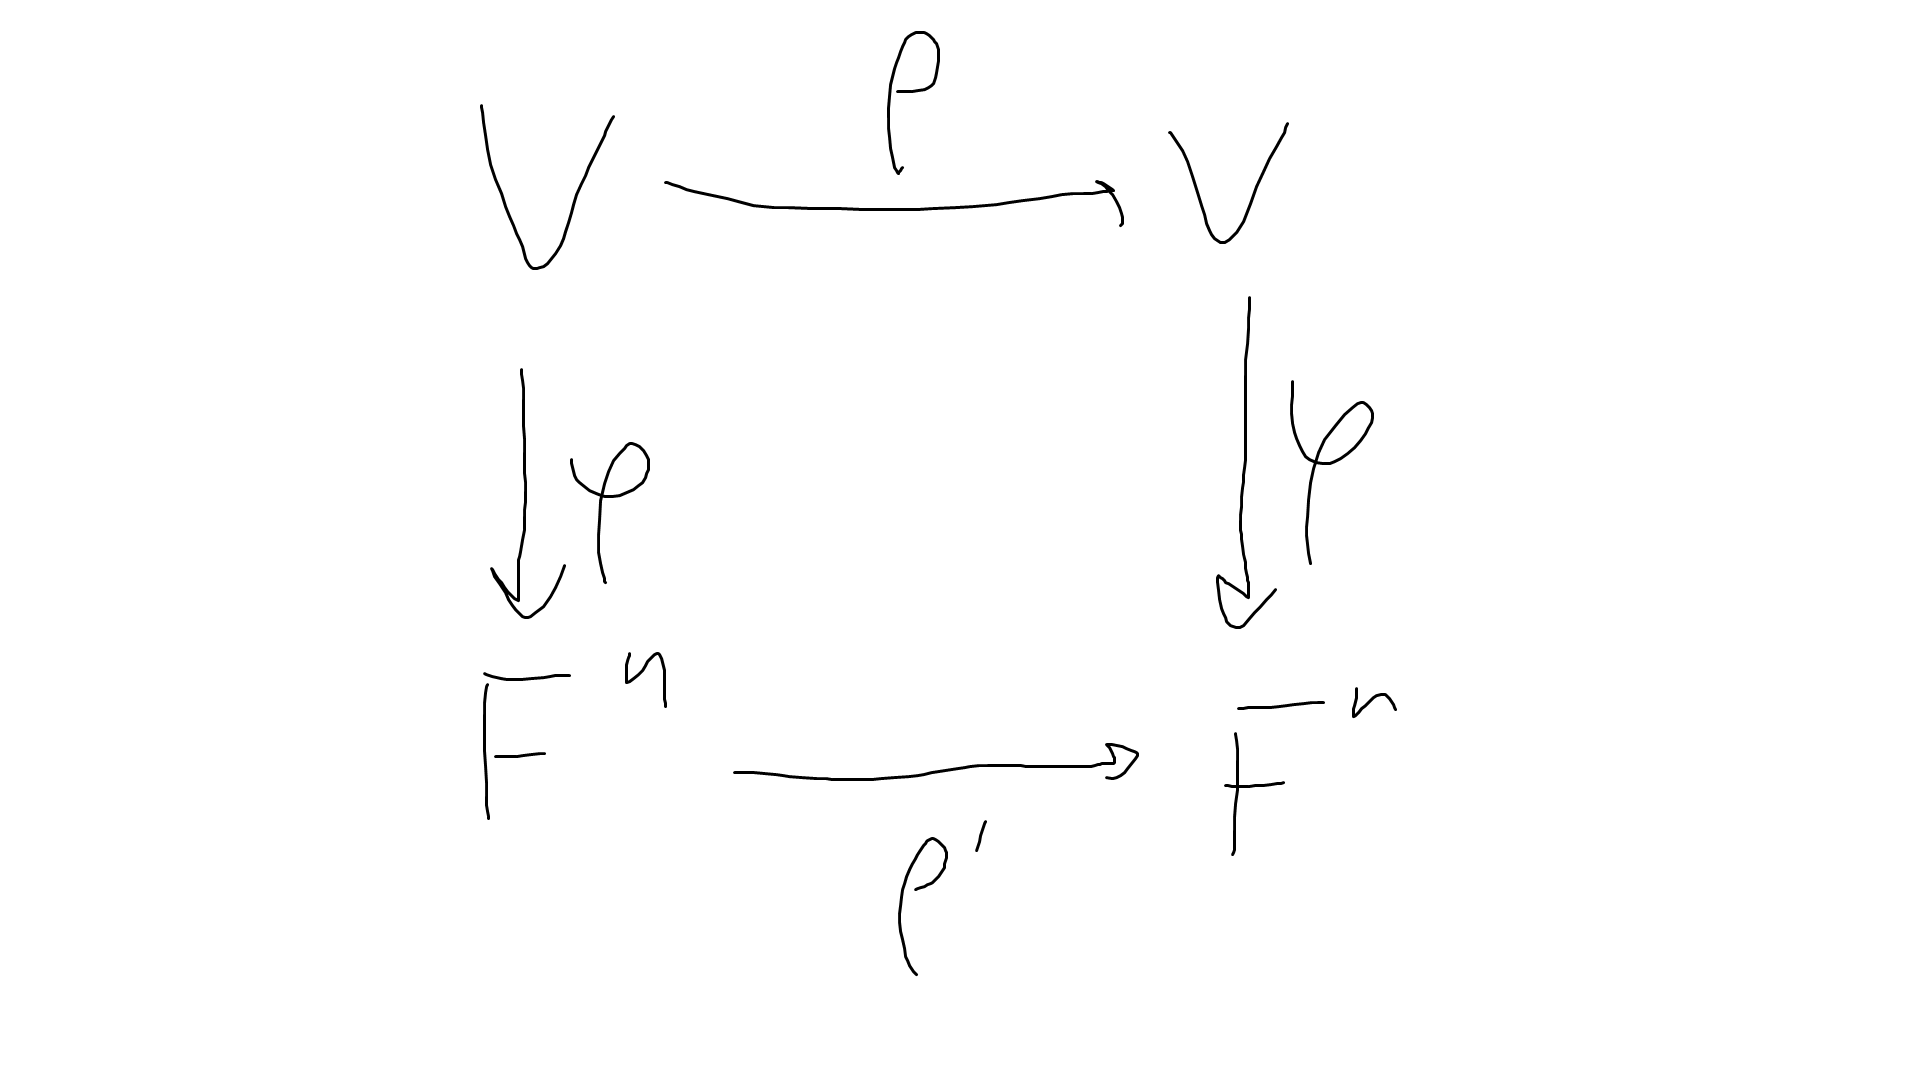
\includegraphics[scale=0.5]{image/Rep_02.png}
\end{rem}

(2.12) In terms of matrix representations, we have
\begin{equation*}
\begin{aligned}
R: G &\to GL_n(F),\\
R':G &\to GL_n(F)
\end{aligned}
\end{equation*}
are ($G$)-isomorphic or equivalent if there exists a nonsingular matrix $X \in GL_n(F)$ with $R'(g) = XR(g)X^{-1}$ $\forall g \in G$.

In terms of linear $G$-actions, the actions of $G$ on $V$,$V'$ are $G$-isomorphic if there exists isomorphisms $\phi:V \to V'$ such that $g:\phi(v) = \phi(gv)$ $\forall v \in V,g \in G$.

\subsection{Subrepresentations}
\begin{defi} (2.13)\\
Let $\rho:G \to GL(V)$ be a representation of $G$. We say $W \leq V$ is a $G$-subspace if it's a subspace and it is $\rho(G)$-invariant, i.e. $\rho_g(W) \leq W \forall g \in G$. Obviously $\{0\}$ and $V$ are $G$-subspaces, however.\\
$\rho$ is \emph{irreducible/simple} representation if there are no proper $G$-subspaces.
\end{defi}

\begin{eg} (2.14)\\
Any $1$-dimensional representation of $G$ is irreducible, but not conversely, e.g. $D_8$ has $2$-dimensional $\C$-irreducible representation.
\end{eg}

(2.15) In definition (2.13), if $W$ is a $G$-subspace, then the corresponding map
\begin{equation*}
\begin{aligned}
G &\to GL(W)\\
g &\to \rho(g)|_W
\end{aligned}
\end{equation*}
is a representation of $G$, a \emph{subrepresentation} of $\rho$.

\begin{lemma} (2.16)\\
In definition (2.13), given $\rho:G \to GL(V)$, if $W$ is a $G$-subspace of $V$ and if $B=\{v_1,...,v_n\}$ is a basis containing basis $B_1 = \{v_1,...,v_m\}$ of $W$ ($0<m<n$) then the matrix of $\rho(g)$ w.r.t. $B$ has block upper triangular form as the graph below, for each $g \in G$.
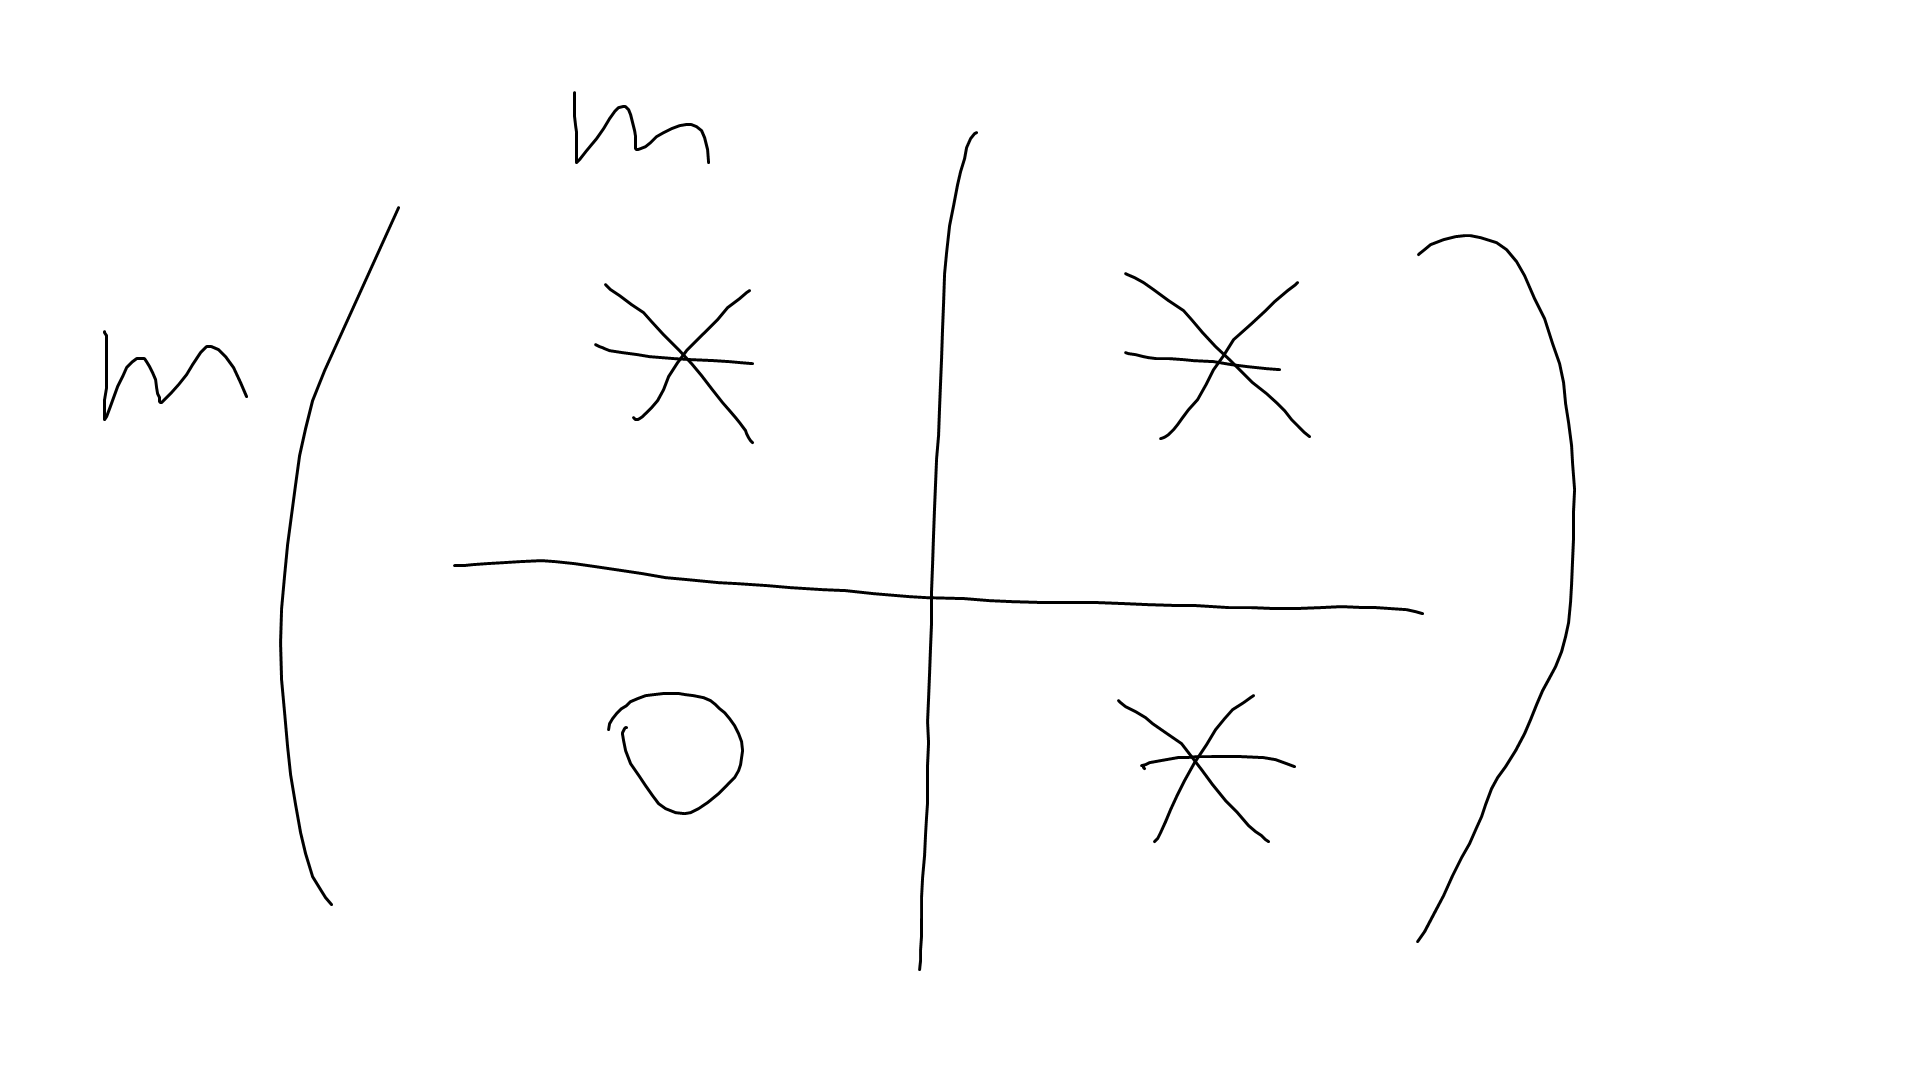
\includegraphics[scale=0.5]{image/Rep_03.png}
\end{lemma}

\begin{eg} (2.17)\\
(i) The irreducible representations of $C_4=\bra x:x^4=1\ket$ are all $1$-dimensional and four of these are $x\to i,x \to -1, x \to -i, x \to 1$. In general, $C_m=\bra x:x^m=1\ket$ has precisely $m$ irreducible complex representations, all of dimension 1. In fact, all complex irreducible representations of a finite abelian group are $1$-dimensional (use (1.4)* or see (4.4) below).\\
(ii) $G=D_6$: any irreducible $C$-representation has dimension $\leq 2$.\\
Let $\rho:G \to GL(V)$ be irreducible $G$-representation. Let $r,s$ be rotation and reflection in $D_6$ respectively. Let $V$ be eigenvector of $\rho(r)$. So $\rho(r) v = \lambda v$ for some $\lambda \neq 0$. Let $W=span\{v,\rho(s)v\} \leq V$. Since $\rho(s)\rho(s)v = v$ and $\rho(r)\rho(s) v = \rho(s)\rho(r)^{-1} v = \lambda^{-1} \rho(s) v$, both of which are in $W$; so $W$ is $G$-invariant, i.e. a $G$-subspace. Since $V$ is irreducible, $W=V$.
\end{eg}

\begin{defi} (2.18)\\
We say at $\rho:G \to GL(V)$ is \emph{decomposable} if there are proper $G$-invariant subspaces $U,W$ with $V = U \oplus W$. Say $\rho$ is direct sum $\rho_U \oplus \rho_W$. If no such decomposition exists, we say that $\rho$ is \emph{indecomposable}.
\end{defi}

\begin{lemma} (2.19)\\
Suppose $\rho:G \to GL(V)$ is decomposable with $G$-invariant decomposition $V=U \oplus W$. If $B$ is a basis $\{\underbrace{u_1,...,u_k}_{B_1}, \underbrace{w_1,...,w_l}_{B_2}\}$ of $V$ consisting of basis of $U$ and basis of $W$, then w.r.t. $B$, $\rho(g)_B$ is a block diagonal matrix $\forall g\in G$ as 
\begin{equation*}
\begin{aligned}
\rho(g)_B = \begin{pmatrix}
[\rho_W(g)]_{B_1} & 0\\
0 & [\rho_W(g)]_{B_2}
\end{pmatrix}
\end{aligned}
\end{equation*}
\end{lemma}

\begin{defi} (2.20)\\
If $\rho:G \to GL(V)$, $\rho':G \to GL(V')$, the \emph{direct sum} of $\rho,\rho'$ is $$\rho \oplus \rho':G \to GL(V \oplus V')$$ where $\rho \oplus \rho'(g) (v_1+v_2) = \rho(g)v_1 + \rho'(g) v_2$, a \emph{block diagonal action}. For matrix representations $R:G \to GL_n(F)$, $R':G \to GL_{n'} (F)$, define $R \oplus R': G \to GL_{n+n'}(F)$:
\begin{equation*}
\begin{aligned}
g \to \begin{pmatrix}
R(g) & 0\\
0 & R'(g)
\end{pmatrix}
\end{aligned}
\end{equation*}
\end{defi}

\newpage
\section{Complete reducibility and Maschke's theorem}
\begin{defi} (3.1)\\
A representation $\rho:G \to GL(V)$ is \emph{completely reducible}, or \emph{semisimple}, if it is a direct sum of irreducible representations. Evidently, irreducible implies completely reducible (lol).
\end{defi}

\begin{rem} (3.2)\\
(1) The converse is false;\\
(2) See sheet 1 Q3: $\C$-representation of $\Z$ is not completely reducible and also representation of $C_p$ over $\F_p$ is not c.r..

Fron now on, take $G$ finite and $char\ F =0$.
\end{rem}

\begin{thm} (3.3)\\
Every f.d. representation $V$ of a finite group over a field of char $0$ is completely reducible, i.e. $$V \cong V_1 \oplus ... \oplus V_r$$is a direct sum of representations, each $V_i$ irreducible.
\end{thm}

It is enough to prove:

\begin{thm} (3.4 Maschke's theorem, 1899)\\
Let $G$ be finite, $\rho:G \to GL(V)$ a f.d. representation, $char\ F = 0$. If $W$ is a $G$-subspace of $V$, then there exists a $G$-subspace $U$ of $V$ s.t. $V = W \oplus U$, a direct sum of $G$-subspaces.
\begin{proof} (1)\\
Let $W'$ be any \emph{vector subspace} complement of $W$ in $V$, i.e. $V=W \oplus W'$ as vector spaces, and $W \cap W'=0$. Let $q:V \to W$ be th projection of $V$ onto $W$ along $W'$ ($\ker q = W'$), i.e. if $v=w+w'$ then $q(v) = w$. Define $$\bar{q} : v \to \frac{1}{|G|} \sum_{g \in G} g q(g^{-1}v)$$the 'average' of $q$ over $G$. Note that in order for $\frac{1}{|G|}$ to exists, we need $char\ F = 0$. It still works if $char\ F \nmid |G|$.\\
Claim (1): $\bar{q}:V \to W$: For $v \in V$, $g(q^{-1}v) \in W$ and $gW \leq W$;\\
Claim (2): $\bar{q}(w) = w$ for $w \in W$: $$\bar{q}(w) = \frac{1}{|G|} \sum_{g \in G} gq(g^{-1}w) = \frac{1}{|G|} \sum g(g^{-1}w) = \frac{1}{|G|} \sum w = w$$
So these two claims imply that $\bar{q}$ projects $V$ onto $W$.\\
Claim (3) If $h \in G$ then $h\bar{q}(v) = \bar{q}(hv)$ ($v \in V$):
\begin{equation*}
\begin{aligned}
h\bar{q}(v) &= h\frac{1}{|G|} \sum_g g \cdot q(g^{-1} v)\\
&= \frac{1}{|G|} \sum_g hgq(g^{-1} v)\\
&= \frac{1}{|G|} \sum (hg) q((hg)^{-1} hv)\\
&= \frac{1}{|G|} \sum_g gq(g^{-1}(hv))\\
&= \bar{q}(hv\\
&= \bar{q}(hv))
\end{aligned}
\end{equation*}
We'll then show that the kernel of this map is $G$-invariant, so this gives a $G$-summand on Thursday.

Let's now show $\ker \bar{q}$ is $G$-invariant. If $v \in \ker \bar{q}$, then $h\bar{q}(v) = 0 = \bar{q}(hv)$, so $hv \in \ker \bar{q}$. Thus $V = im \bar{q} \oplus \ker \bar{q} = W \oplus \ker \bar{q}$ is a $G$-subspace decomposition.

We can deduce (3.3) from (3.4) by induction on $\dim V$. If $\dim V = 0$ or $V$ is irreducible, then result is clear. Otherwise, $V$ has non-trivial $G$-invariant subspace, $W$. Then by (3.4), there exists $G$-invariant complement $U$ s.t. $V = U \oplus W$ as representations of $G$. But $\dim U, \dim W < \dim V$. So by induction they can be broken up into direct sum of irreducible subrepresentations.
\end{proof}

The second proof uses inner products, hence we need to take $F = \C$ and can be generalised to compact groups in section 15.\\
Recall, for $V$ a $\C$-space, $\bra,\ket$ is a \emph{Hermitian inner product} if\\
(a) $\bra w,v\ket =\overline{\bra v,w\ket}$ $\forall v,w$ (Hermitian);\\
(b) linear in RHS (sesquilinear);\\
(c) $\bra v,v\ket > 0$ iff $v \neq 0$ (positvie definite).

Additionally, $\bra,\ket$ is \emph{G-invariant} if \\
(d) $\bra gv,gw\ket = \bra v,w\ket$ $\forall v,w \in V, g \in G$.

Note if $W$ is $G$-invariant subspace of $V$, with $G$-invariant inner product, then $W^\perp$ is also $G$-invariant, and $V \oplus W^\perp$. For all $v \in W^\perp$, $g \in G$, we have to show that $gv \in W^\perp$. But $v \in W^\perp \iff \bra v,w\ket = 0 \forall w \in W$. Thus by (d), $\bra gv,gw\ket = 0$ $\forall g \in G \forall w \in W$. Hence $\bra gv,w'\ket = 0$ $\forall w' \in W$. Since we can choose $w=g^{-1}w' \in W$ by $G$-invariance of $W$. Thus $gv \in W^\perp$ since $g$ was arbitrary.

Hence if there is a $G$-invariant inner product on any $G$-space, we get another proof of Maschke's theorem:

(3.4*) (Weyl's unitary trick)\\
Let $\rho$ be a complex representation of the finite group $G$ on the $\C$-space $V$. Then there is a $G$-invariant Hermitian inner product on $V$.
\begin{rem}
Recall the \emph{unitary group} $U(V)$ on $V$: $\{f \in GL(V): (fu,fv) = (u,v) \forall u,v \in V\} = \{A \in GL_n(\C) : A \bar{A}^T = I\} (= U(n))$ by choosing orthonormal basis.\\
Sheet 1 Q.12: any finite subgroup of $GL_n(\C)$ is conjugate to a subgroup of $U(n)$.
\end{rem}

\begin{proof} (2)\\
There exist an inner product on $V$: take basis $e_1,...,e_n$ and define $(e_i,e_j) = \delta_{ij}$, extended sesquilinearly. Now
\begin{equation*}
\begin{aligned}
\bra v,w\ket := \frac{1}{|G|} \sum_{g \in G} (gv,gw)
\end{aligned}
\end{equation*}
we claim that $\bra,\ket$ is sesquilinear, positive definite and $G$-invariant: if $h \in G$, then
\begin{equation*}
\begin{aligned}
\bra hv,hw\ket = \frac{1}{|G|} \sum_{g \in G} ((gh)v,(gh)w)\\
&= \frac{1}{|G|} \sum_{g' \in G} (g'v, g'w)\\
&= \bra v,w\ket
\end{aligned}
\end{equation*}
for all $v,w \in V$.
\end{proof}
\end{thm}

\begin{defi} (3.5, the regular representation)\\
Recall \emph{group algebra} of $G$ is $F$-space $FG = span\{e_g:g \in G\}$. There is a linear $G$-action
\begin{equation*}
\begin{aligned}
h \in G, h \sum_{g \in G} a_g e_g = \sum_{g \in G} a_g e_{hg} (=\sum_{g' \in G} a_{h^{-1} g'} e_{g'})
\end{aligned}
\end{equation*}
$\rho_{reg}$ is the corresponding representation, the \emph{regular representation} of $G$. This is faithful of $\dim |G|$. $FG$ is the \emph{regular module}.
\end{defi}

\begin{prop}
Let $\rho$ be an irreducible representation of $G$ over a field of characteristic 0. Then $\rho$ is isomorphic to a subrepresentation of $\rho_{reg}$.
\begin{proof}
Take $\rho: G \in GL(V)$ irreducible and let $0 \neq v \in V$. Let $\theta : FG \to V$ by $\sum a_g e_g \to \sum a_g gv$. Check this is a $G$-homomorphism. Now $V$ is irreducible so $im\theta = V$ (since $im\theta$ is a $G$-subspace).

Also $\ker\theta$ is $G$-subspace of $FG$. Let $W$ be $G$-complement of $\ker \theta$ in $FG$ (Maschke), so that $W < FG$ is $G$-subspace and $FG = \ker\theta \oplus W$. Thus $W \cong FG/\ker \theta \cong(G-isomorphism) im\theta \cong V$.
\end{proof}
\end{prop}

More generally,
\begin{defi} (3.7)\\
Let $F$ be a field. Let $G$ act on set $X$. Let $FX = span\{e_x:x \in X\}$ with $G$-action
\begin{equation*}
\begin{aligned}
g(\sum a_x e_x) = \sum a_x e_{gx}
\end{aligned}
\end{equation*}
\end{defi}

The representation $G \to GL(V)$ where $V=FX$ is the corresponding \emph{permutation representation}. See section 7.

\newpage

\section{Schur's lemma}
It's really unfair that such an important result is only remembered by a lemma, so we shall call it a theorem.
\begin{thm} (4.1, Schur)\\
(a) Assume $V,W$ are irreducible $G$-spaces over field $F$. Then any $G$-homomorphism $\theta:V \to W$ is either $0$ or an isomorphism.\\
(b) Assume $F$ is \emph{algebraically closed}, and let $V$ be an irreducible $G$-space. Then any $G$-endomorphism $V \to V$ is a scalar multiple of the identity map $\iota_V$.
\begin{proof}
(a) Let $\theta:V \to W$ be a $G$-homomorphism. Then $\ker$ $\theta$ is $G$ subspace of $V$ and, since $V$ is irreducible, we get $\ker\theta = 0$ or $\ker\theta = V$.\\
And $im\theta$ is $G$-subspace of $W$, so as $W$ is irreducible, $im\theta$ is either $0$ or $W$. Hence, either $\theta=0$ or $\theta$ is injective and surjective, hence isomorphism.\\
(b) Since $F$ is algebraically closed, $\theta$ has an eigenvalue, $\lambda$. Then $\theta-\lambda \iota$ is singular $G$-endomorphism of $V$, but it cannot be an isomorphism, so it is $0$ (by (a)). So $\theta = \lambda \iota_V$.
\end{proof}
\end{thm}

Recall from (2.8), the $F$-space $Hom_G(V,W)$ of all $G$-homomorphisms $V \to W$. Write $End_G(V)$ for the $G$-endomorphisms of $V$.

\begin{coro} (4.2)\\
If $V,W$ are irreducible complex $G$-spaces, then
\begin{equation*}
\begin{aligned}
\dim_\C Hom_G (V,W) = \left\{\begin{array}{ll}
1 & \text{ if } V,W \text{ are } G- \text{ isomorphic}\\
0 & \text{ otherwise}
\end{array}
\right.
\end{aligned}
\end{equation*}
\begin{proof}
If $V,W$ are not $G$-isomorphic then the only $G$-homomorphism $V\to W$ is $0$ by (4.1). Assume $v \cong_G W$ and $\theta_1,\theta-2 \in Hom_G (V,W)$, both non-zero. Then $\theta_2$ is invertible by (4.1), and $\theta_2^{-1} \theta_1 \in End_G(V)$, and non-zero, so $\theta_2^{-1} \theta_1 = \lambda\iota_V$ for some $\lambda \in \C$. Hence $\theta_1 = \lambda\theta_2$.
\end{proof}
\end{coro}

\begin{coro} (4.3)\\
If finite group $G$ has a faithful complex irreducible representation, then $Z(G)$, the centre of the group, is cyclic.\\
Note that the converse is false (Sheet 1, Q10).
\begin{proof}
Let $\rho:G \to GL(V)$ be faithful irreducible complex representation. Let $z \in Z(G)$, so $zg = gz$ $\forall g \in G$, hence the map $\phi_z: v \to z(v)$ ($v \in V$) is $G$-endomorphism of $V$, hence is multiplication by scalar $\mu_z$, say.\\
By Schur's lemma, $z(v) = \mu_z v$ $\forall v$. Then the map 
\begin{equation*}
\begin{aligned}
Z(G) &\to \C^* \ (\text{multiplicative group})\\
z &\to \mu_z
\end{aligned}
\end{equation*}
is a representation of $Z$ and is faithful, since $\rho$ is. Thus $Z(G)$ is isomorphic to some finite subgroup of $\C^*$, so is cyclic.
\end{proof}
\end{coro}

Let's now consider representation of finite abelian groups.

\begin{coro} (4.4)\\
The irreducible $\C$-representations of a finite abelian group are all $1$-dimensional.
\begin{proof}
\emph{Either}: use (1.4)* to invoke simultaneous diagonalisation: if $v$ is an eigenvector for each $g \in G$, and if $V$ is irreducible, then $V=\bra v\ket$.\\
\emph{Or}: Let $V$ be an irreducible $\C$-representation. For $g \in G$, the map
\begin{equation*}
\begin{aligned}
\theta_g: &V &\to v\\
&v &\to gv
\end{aligned}
\end{equation*}
is a $G$-endomorphism of $V$, and as $V$ irreducible, $\theta_g = \lambda_g \iota_V$ for some $\lambda_g \in \C$. Thus $gv = \lambda_g v$ for any $g \in G$ (so $\bra v\ket$ is a $G$-subspace of $V$). Thus as $0 \neq V$ is irreducible, $V = \bra v\ket$, which is $1$-dimensional.
\end{proof}
\end{coro}

\begin{rem}
Schur's lemma fails over non-algebraically closed field, in particular, over $\R$. For example, let's consider the cyclic group $C_3$. It has 2 irreducible $\R$-representations, one of dimension 1 (maps everything to 1) and one of dimension 2(imo consider $\C$ as a dimension 2 space over $\R$, then map the generator to the 3rd root of unity?) (so 'contradicting' with Schur's lemma via the corollary above).\\
Recall that every finite abelian group $G$ is isomorphic to a product of cyclic groups (see GRM). For example, $C_6 = C_2 \times C_3$. In fact, it can be written as a product of $C_{p^\alpha}$ for various primes $p$ and $\alpha \geq 1$, and the factors are uniquely determined up to reordering.
\end{rem}

\begin{prop} (4.5)\\
The finite abelian group $G=C_{n_1} \times ... \times C_{n_r}$ has precisely $|G|$ irreducible $\C$-representations, as described below:
\begin{proof}
Write $G = \bra x_1\ket \times ... \bra x_r\ket$ where $|x_j| = n_j$. Suppose $\rho$ is irreducible, so by (4.4), it's $1$-dimensional: $\rho:G \to \C^*$.\\
Let $\rho(1,...,x_j,...,1)$ (all $1$ apart from the $j^{th}$ entry) be $\lambda_j$. Then $\lambda_j^{n_j} = 1$, so $\lambda_j$ is a $n_j$-th root of unity. Now, the values $(\lambda_1,...,\lambda_r)$ determine $\rho$: $$\rho(x_1^{j_1}, ..., x_r^{j_r}) = \lambda_1^{j_1}...\lambda_r^{j_r}$$
thus $\rho \leftrightarrow (\lambda_1,...,\lambda_r)$ with $\lambda_j^{n_j} =1 $ $\forall j$; we have $n_1...n_r$ such $r$-tuples, each giving $1$-dimensional representation.
\end{proof}
\end{prop}

\begin{eg} (4.6)\\
Consider $G=C_4 = \bra x\ket$. We could have $\rho_1(x) = 1,\rho_2(x) = i,\rho_3(x)=-1,\rho_4(x)=-i$.
\end{eg}

Warning: There is no "natural" 1-1 correspondence between the elements of $G$ and the representations of $G$ ($G$-finite abelian). If you choose an isomorphism $G \cong C_{a_1} \times ... \times C_{a_r}$, then we can identify the two sets (elements of groups and representations of $G$), but it depends on the choice of isomorphism.

Isotypical decomposition:

Recall any diagonalisable endomorphism $\alpha:V \to V$ gives eigenspace decomposition of $V \cong \oplus_\lambda V(\lambda)$, where $V(\lambda) = \{v:\alpha v = \lambda v\}$. This is \emph{caconical} (one of the three useless words: \emph{arbitrary}(anything), \emph{canonical}(only one choice), \emph{uniform}(you can choose, but it doesn't really matter)), in the sense that it depends on $\alpha$ alone (and nothing else).\\
There is no canonical eigenbasis of $V$: must choose basis in each $V(\lambda)$.

We know that in $char\ 0$ every representation $V$ decomposes as $\oplus n_i V_i$, $V_i$ irreducible, $n_i \geq 0$. How unique is this?

We have this wishlist (4.7):\\
(a) Uniqueness: for each $V$ there is only one way to decompose $V$ as above. However, this doesn't work obviously.\\
(b) Isotypes: for each $V$, there exists a unique collection of subrepresentations $U_1,...,U_k$ s.t. $V=\oplus U_i$ and, if $V_i \subseteq U_i$ and $V'_j \subseteq U_j$ are irreducible subrepresentations, then $V_i \cong V'_j$ iff $i = j$.\\
(c) Uniqueness of factors: If $\oplus_{i=1}^k V_i \cong \oplus_{i=1}^k V'_i$ with $V_i,V'_i$ irreducible, then $k=k'$, and $\exists \pi \in S_k$ such that $V'_{\pi(i)} \cong V_i$ (Krull-Schimdt theorem).\
For (b),(c) see Teleman section 5.

\begin{lemma} (4.8)\\
Let $V,V_1,V_2$ be $G-$spaces over $F$.\\
(i) $Hom_G(V,V_1 \oplus V_2) \cong Hom_G (V,V_1) \oplus Hom_G(V,V_2)$;\\
(ii) $Hom_G(V_1\oplus V_2, V) \cong Hom_G(V_1,V) \oplus Hom_G(V_2,V)$;\\
\begin{proof}
(i) Let $\pi_i: V_1 \oplus V_2 \to V_i$ be $G$-linear projections onto $V_i$, with kernel $V_{3-i}$ ($i=1,2$).\\
Consider 
\begin{equation*}
\begin{aligned}
Hom_G (V,V_1 \oplus V_2) &\to Hom_G (V,V_1) \oplus Hom_G (V,V_2)\\
\phi &\to (\pi_1 \phi, \pi_2 \phi)
\end{aligned}
\end{equation*}
This map has inverse $(\psi_1,\psi_2) \to \psi_1+\psi_2)$. Check details.\\
(ii) The map $\phi \to (\phi|_{V_1},\phi|_{V_2})$ has inverse $(\psi_1,\psi_2) \to \psi_1\pi_1+\psi_2\pi_2$.
\end{proof}
\end{lemma}

\begin{lemma}
Let $F$ be algebraically closed, $V=\oplus_1^n V_i$ a decomposition of $G$-space into irreducible summands. Then, for each irreducible representation $S$ of $G$,
\begin{equation*}
\begin{aligned}
\#\{j:V_j \cong S\} = \dim Hom_G(S,V)
\end{aligned}
\end{equation*}
where $\#$ means 'number of times'. This is called the \emph{multiplicity} of $S$ in $V$.
\begin{proof}
Indunction on $n$. $n=0,1$ are trivial.\\
If $n>1$, $V=\oplus_1^{n-1} V_i \oplus V_n$. By (4.8) we have
\begin{equation*}
\begin{aligned}
\dim Hom_G (S,\oplus_1^{n-1} V_i \oplus V_n) = \dim Hom(S,\oplus_1^{n-1} V_i) + \underbrace{\dim Hom_G (S,V_n)}_{\text{Schur's lemma}}
\end{aligned}
\end{equation*}
\end{proof}
\end{lemma}

\begin{defi} (4.10)\\
A decomposition of $V$ as $\oplus W_j$ where each $W_j \cong n_j$ copies of irreducible representations $S_j$ (each non-isomorphic for each $j$) is the \emph{canonical decomposition} or the decomposition into \emph{isotypical components} $W_j$. For $F$ algebraically closed, $n_j=\dim Hom_G(S_j,V)$.
\end{defi}

\newpage

\section{Character theory}

We want to attach invariants to representation $\rho$ of a finite group $G$ on $V$. Matrix coefficients of $\rho(g)$ are basis dependent, so not true invariants.\\
Let's take $F=\C$, $G$ finite, $\rho=\rho_V: G \to GL(V)$ be a representation of $G$.

\begin{defi} (5.1)\\
The \emph{character} $\chi_\rho = \chi_V = \chi$ is defined as $\chi(g) = \tr \rho(g) = \tr R(g)$ where $R(g)$ is any matrix representation of $\rho(g)$ w.r.t. any basis.\\
The degree of $\chi_V$ is $\dim_\C V$.\\
Thus $\chi$ is a function $G \to \C$. $\chi$ is \emph{linear} (not a universal name) if $\dim V=1$, in which case $\chi$ is a homomorphism $G \to \C^*$ ($=GL_1(\C)$).\\
$\chi$ is irreducible if $\rho$ is; $\chi$ is faithful if $\rho$ is; and, $\chi$ is trivial, or principal, if $\rho$ is the trivial representation (2.6). We write $\chi = 1_G$ in that case.\\
$\chi$ is a complete invariant in the sense that it determines $\rho$ up to isomorphism -- see (5.7).
\end{defi}

\begin{thm} (5.2, first properties)\\
(i) $\chi_V(1) = \dim_\C V$; (clear: $\tr I_n = n$)\\
(ii) $\chi_V$ is a \emph{class function}, via it is conjugation-invariant: $$\chi_V (hgh^{-1}) = \chi_V(g) \forall g,h \in G$$
Thus $\chi_V$ is constant on conjugacy classes.\\
(iii) $\chi_V(g^{-1}) = \overline{\chi_V(g)}$, the complex conjugate;\\
(iv) For two representations $V,W$, $\chi_{V \oplus W} = \chi_V + \chi_W$.
\begin{proof}
(ii) $\chi(hgh^{-1}) = \tr (R_h R_g R^{-1}_h) = \tr (R_g) = \chi(g)$.\\
(iii) Recall $g \in G$ has finite order, so we can assume $\rho(g)$ is represented by a diagonal matrix $Diag(\lambda_1,...,\lambda_n)$. Then $\chi(g) = \sum \lambda_i$. Now $g^{-1}$ is represented by the matrix $Diag(\lambda_1^{-1},...\lambda_n^{-1})$, and hence $\chi(g^{-1}) = \sum \lambda_i^{-1} = \sum \bar{\lambda_i} = \overline{\chi(g)}$ (since $\lambda_i$'s are roots of unity -- since $g^k = 1$ for some $k$!(I mean an exclamation mark here to express surprise) and by homomorphism we know that).\\
(iv) Suppose $V = V_1 \oplus V_2$, $\rho_i : G \to GL(V_i)$, $\rho:G \to GL(V)$. Take basis $B = B_1 \cup B_2$ of $V$ w.r.t $B$, $\rho(g)$ has matrix of block form $Diag([\rho_1(g)]_{B_1},[\rho_2(g)]_{B_2})$ and as $\chi(g)$ is the trace of the above matrix, it is equal ot $\tr \rho_1(g)+ \tr\rho_2(g) = \chi_{\rho_1} (g) + \chi_{\rho_2}(g)$.
\end{proof}
\end{thm}

\begin{rem}
We see later that $\chi_1,\chi_2$ character of $G$ implies that $\chi_1\chi_2$ is also a character of $G$: uses tensor products, see (9.6).
\end{rem}

\begin{lemma} (5.3)\\
Let $\rho:G \to GL(V)$ be a copmlex representation \emph{affording} the character $\chi$ (i.e. $\chi$ is a character of $\rho$). Then $|\chi(g)| \leq \chi(1)$, with equality iff $\rho(g) = \lambda_I$ for some $\lambda \in \C$, a root of unity. Moreover, $\chi(g) = \chi(1)$ iff $g \in \ker \rho$.
\begin{proof}
Fix $g$. W.r.t. basis of $V$ of eigenvalues $\rho(g)$, the matrix of $\rho(g)$ is $Diag(\lambda_1,...,\lambda_n)$. Hence $|\chi(g)| = |\sum \lambda_j| \leq \sum |\lambda_j|= \sum 1 = \dim V = \chi(1)$. Equality holds iff all $\lambda_j$ are equal (to $\lambda$, say).\\
If $\chi(g) = \chi(1)$, then $\rho(g) = \lambda \iota$ has $\chi(g) = \lambda \chi(1)$.
\end{proof}
\end{lemma}

\begin{lemma} (5.4)\\
(a) If $\chi$ is a complex irreducible character of $G$, so is $\bar{\chi}$;\\
(b) Under the same assumption, so is $\varepsilon\chi$ for any linear character $\varepsilon$ of $G$.\
\begin{proof}
If $R:G \to GL_n (\C)$ is a complex irreducible representation then so is $\bar{R}: G \to GL_n (\C)$ by $g \to \bar{R}(g)$. Similarly for $R': g \to \varepsilon(g) R(g)$ for $g \in G$. Check the details.
\end{proof}
\end{lemma}

\begin{defi} (5.5)\\
$\mathcal{C}(G) = \{f: G \to \C: f(hgh^{-1}) = f(g) \forall h,g \in G\}$, the $\C$-space of class functions (we call it a space since $f_1+f_2: g \to f_1(g)+f_2(g)$, $\lambda f: g \to \lambda f(g)$ are still in $\mathcal{C}(G)$), so this is a vector space.\\
Let $k = k(G)$ be the number of ccls of $G$. List the ccls $\mathcal{C}_1,...,\mathcal{C}_k$. Conventionally we choose $g_1 = 1, g_2,...,g_k$, representatives of the ccls (hence $\mathcal{C}_1 = \{1\}$). Note that $\dim_\C \mathcal{C}(G) = k$ (the characteristic functions $\delta_j$ of each ccl which maps any element in the ccl to 1 and others to 0 form a basis).\\
We define Hermitian inner product on $\mathcal{C}(G)$:
\begin{equation*}
\begin{aligned}
\bra f,f' \ket &= \frac{1}{|G|} \sum_{g \in G} \overline{f(G)} f'(g)\\
&= \frac{1}{|G|} \sum_{j=1}^k |\mathcal{C}_j| \overline{f(g_j)} f'(g_j)\\
&= \sum_{j=1}^k \frac{1}{|C_G(g_j)} \overline{f(g_j)} f'(g_j)
\end{aligned}
\end{equation*}
using $|\mathcal{C}_x| =  |G:C_g(x)|$, where $\mathcal{C}_x$ is the ccl of $x$, $C_G(x)$ is the centraliser of $x$.\\
For characters
\begin{equation*}
\begin{aligned}
\bra \chi,\chi' \ket &= \sum \frac{1}{|C_G(g_j)|} \chi(g_j^{-1}) \chi'(g_j)
\end{aligned}
\end{equation*}
is a real symmetric form (in fact, $\bra \chi,\chi'\ket \in \Z$ -- see later).
\end{defi}

\begin{thm} (5.6)\\
The $\C$-irreducible characters of $G$ form an orthonormal basis of $\mathcal{C}(G)$. Moreover,\\
(a) If $\rho:G \to GL(V), \rho': G \to GL(V')$ are irreducible representations of $G$ affording characters $\chi,\chi'$ respecitvely, then
\begin{equation*}
\begin{aligned}
\bra \chi,\chi' \ket = \left\{\begin{array}{ll}
1 & \rho,\rho' \text{ are isomorphic representations}\\
0 & \text{ otherwise}
\end{array}
\right.
\end{aligned}
\end{equation*}
we call this 'row orthogonality'.\\
(b) Each class function of $G$ can be expressed as a linear combination of $G$.\\
This will be proved later in section 6.
\end{thm}

\begin{coro} (5.7)\\
Complex representations of \emph{finite} groups are characterised by their characters.\\
We emphasise on finiteness here: for example, $G=\Z$, consider $1 \to I_2$, $1 \to {{1\ 1} \choose {0\ 1}}$ are non-isomorphic but have same character.
\begin{proof}
Let $\rho:G \to GL(V)$ be representation affording $\chi$ ($G$ finite over $\C$). (3.3) says 
\begin{equation*}
\begin{aligned}
\rho = m_1 \rho_1 \oplus ... \oplus m_k \rho_k
\end{aligned}
\end{equation*}
where $\rho_1,...,\rho_k$ are irreducible, and $m_j \geq 0$. Then $m_j = \bra \chi,\chi_j\ket$ where $\chi_j$ is afforded by $\rho_j$: we have $\chi = m_1\chi_1 + ... + m_k \chi_k$, but the $\rho_i$'s are orthonormal.
\end{proof}
\end{coro}

\begin{coro} (5.8, irreduciblility criterion)\\
If $\rho$ is $\C$-representation of $G$ affording $\chi$, then $\rho$ irreducible $\iff$ $\bra \chi,\chi \ket = 1$.
\begin{proof}
Forward is just the statement of orthonormality. Conversely, assume $bra \chi,\chi\ket = 1$. Now take a (complete) decomposition of $\rho$ and take characters of it we get $\chi = \sum m_j \chi_j$ with $\chi_j$ irreducible and $m_j \geq 0$. Then $\sum m^2_j = 1$. Hence $\chi = \chi_j$ for some $j$ (since the $m_j$'s are obviously integers), so is irreducible.
\end{proof}
\end{coro}

\begin{coro} (5.9)\\
If the irreducible $\C$-representations of $G$ are $\rho_1,...,\rho_k$ have dimensions $n_1,...,n_k$, then 
\begin{equation*}
\begin{aligned}
|G| = \sum_{i=1}^k n_i^2
\end{aligned}
\end{equation*}
\begin{proof}
Recall from (3.5), $\rho_{reg}; G \to GL(\C G)$, the regular representation $G$ of dimension $|G|$ (where $\C G$ is just a $G$-space with basis $\{e_g: g \in G\}$ and any $h \in G$ permutes the $e_g$: $e_g \to e_{hg}$).\\
Let $\pi_{reg}$ be its charcter, the \emph{regular character} of $G$.\\
Claim 1: $\pi_{reg}(1) = |G|$, $\pi_{reg}(h) = 0$ if $h \neq 1$.\\
This is clear: take $h \in G, h \neq 1$, then we always have $0$ down the diagonal since $h$ permutes things around, so the trace is 0; if $h=1$ then we have an identity matrix so trace is $\dim \rho = |G|$.\\
Claim 2: $\pi_{reg} = \sum n_j \chi_j$ with $n_j = \chi_j(1)$.\\
This is because
\begin{equation*}
\begin{aligned}
n_j &= \bra \pi_{reg}, \chi_j\ket\\
&= \frac{1}{|G|} \sum_{g \in G} \overline{\pi_{reg}(g)} \chi_j(g)\\
&= \frac{1}{|G|} \cdot |G| \chi_j(1) = \chi_j(1)
\end{aligned}
\end{equation*}
(all the other $\pi_{reg}(g)$ are zero by claim 1).\\
Our corollary is then obvious by just calculating $|G| = \pi_{reg}(1)$.
\end{proof}
\end{coro}

\begin{coro} (5.10)\\
Number of irreducible characters of $G$ (up to equivalence) = $k$ (=number of ccls).
\end{coro}

\begin{coro} (5.11)\\
Elements $g_1,g_2 \in G$ are conjugate iff $\chi(g_1) = \chi(g_2)$ for all irreducible characters of $G$.
\begin{proof}
Forward: characters are class functions;\\
Backward: Let $\delta$ be the characteristic function of the class of $g_1$. In particular, $\delta$ is a class function, so can be written as a linear combination of the irreducible characters of $G$. Hence $\delta(g_2) = \delta(g_1) = 1$, so $g_2 \in \mathcal{C}_G (g_1)$.
\end{proof}
\end{coro}

In the end let's introduce a good friend which will be around for the next few lectures:\\
Recall from (5.5), the inner product on $\mathcal{C}(G)$ and the real symmetric form $\bra,\ket$ on characters:
\begin{defi}
The \emph{character table} of $G$ is the $k \times k$ matrix (where $k$ is the number of ccls) $X = [\chi_i (g_j)]$, the $i^{th}$ character on the $j^{th}$ class, where we let $\chi_1 =1_G, \chi_2,...,\chi_k$ are the irreducible characters of $G$, and $\mathcal{C}_1 =\{1\},...,\mathcal{C}_k$ are the ccls with $g_j \in \mathcal{C}_j$ (as we defined in 5.5).\\
So the $(i,j)^{th}$ entry of $X$ is just $\chi_i (g_j)$.
\end{defi}

\begin{eg} (5.13)\\
(a) $C_3 = \bra x:x^3=1\ket$. The character table is
\begin{equation*}
\begin{aligned}
\begin{matrix}
 & 1 & x & x^2\\
\chi_1 & 1 & 1 & 1\\
\chi_2 & 1 & \omega & \omega^2\\
\chi_3 & 1 & \omega^2 & \omega
\end{matrix}
\end{aligned}
\end{equation*}
where $\omega = e^{2\pi i/3}$.\\
(b) $G=D_6 \cong S_3 = \bra r,s:r^3=s^2=1,sr^{-1} = r^{-1}\ket$.\\
ccls of $G$: $\mathcal{C}_1 = \{1\}$, $\mathcal{C}_2 = \{r,r^{-1}$, $\mathcal{C}_3 =\{s,sr,sr^2\}$. We have 3 irreducible representations over $\C$: $1_G$ (trivial); $\mathcal{S}$ (sign): $x \to 1$ for $x$ even, $x \to -1$ for $x$ odd; and $W$ (2-dimensional): $sr^i$ acts by matrix with eigenvalues $\pm 1$; $r^k$ acts by the matrix
\begin{equation*}
\begin{aligned}
\begin{matrix}
\cos 2k\pi/3 & -\sin 2k\pi/3\\
\sin 2k\pi/3 & \cos 2k\pi/3
\end{matrix}
\end{aligned}
\end{equation*}
so $\chi_w(sr^i) = 0$ $\forall j$, $\chi_w (r^k) = 2\cos 2k\pi/3 = -1$ $\forall k$. So the charactable is:
\begin{equation*}
\begin{aligned}
\begin{matrix}
 & \mathcal{C}_1 & \mathcal{C}_2 & \mathcal{C}_3\\
 1_G & 1 & 1 & 1\\
 \chi_s & 1 & -1 & 1\\
 \chi_w & 2 & 0 & -1
\end{matrix}
\end{aligned}
\end{equation*}
\end{eg}

\newpage

\section{Proofs and orthogonality}

We want to prove(5.6): irreducible characters form orthonormal basis for the space of $\C$-class functions.

\begin{proof} (of 5.6 (a))\\
Fix bases of $V$ and $V'$. Write $R(g)$, $R'(g)$ for matrices of $\rho(g),\rho'(g)$ w.r.t. these bases, respectively. Then
\begin{equation*}
\begin{aligned}
\bra \chi',\chi \ket &= \frac{1}{|G|} \chi'(g^{-1}) \chi(g) \\
&= \frac{1}{|G|} \sum_{g \in G, i,j\ s.t. 1 \leq i \leq n', 1 \leq j \leq n} R'(g^{-1})_{ii} R(g)_{jj}
\end{aligned}
\end{equation*}
the trick is to define something that annhilates almost the whole thing. Let $\phi:V \to V'$ be linear and define 
\begin{equation*}
\begin{aligned}
\tilde{\phi}: V &\to &V'\\
v &\to &\frac{1}{|G|} \sum_{g \in G} \rho'(g^{-1}) \phi \rho(g) v
\end{aligned}
\end{equation*}
We claim that this is a $G$-homomorphism: if $h \in G$, let's calculate
\begin{equation*}
\begin{aligned}
\rho'(h^{-1}) \tilde{\phi} \rho(h) (v) &= \frac{1}{|G|} \sum_{g \in G} \rho' (gh)^{-1} \phi \rho(gh) (v)\\
&= \frac{1}{|G|} \sum_{g' \in G} \rho'(g'^{-1}) \phi \rho(g') (v)\\
&= \tilde{\phi} (v)
\end{aligned}
\end{equation*}
(when $g$ runs through $G$, $gh$ runs through $G$ as well). So (2.8) is satisfied, i.e. $\phi$ is a $G$-homomorphism.

Case 1: $\rho,\rho'$ are not isomorphic. Schur's lemma says $\tilde{\phi} = 0$ for any given linear $\phi:V \to V'$. Take $\phi - \varepsilon_{\alpha\beta}$, having matrix $E_{\alpha\beta}$ (w.r.t our basis). This is $0$ everywhere except $1$ in the $(\alpha,\beta)$-position. Then $\tilde{\varepsilon_{\alpha\beta}} = 0$. So $\frac{1}{|G|} \sum_{g \in G} (R'(g^{-1}) E_{\alpha\beta} R(g))_{ij} = 0$. So $\frac{1}{|G|} \sum R'(G^{-1})_{i\alpha} R(g)_{\beta j} =0 $ $\forall i,j$, with $\alpha = i, \beta = j$. Now $\frac{1}{|G|} \sum_{g \in G} R'(g^{-1})_{ii} R(g)_{jj} = 0$ sum over $i,j$. Then $\bra \chi',\chi\ket = 0$.\\
Case 2: $\rho,\rho'$ isomorphic. So $\chi = \chi'$; take $V=V'$, $\rho = \rho'$. If $\phi:V \to V$ is linear endomorphism, we claim $\tr \phi = \tr \tilde{\phi}$:
\begin{equation*}
\begin{aligned}
\tr \tilde{\phi} = \frac{1}{|G|} \sum_{g \in G} \tr(\rho(g)^{-1} \phi \rho(g)) = \frac{1}{|G|} \sum_{g \in G} \tr \phi = \tr \phi
\end{aligned}
\end{equation*}
By Schur's lemma, $\tilde{\phi} = \lambda\iota_V$ for some $\lambda \in \C$ (depending on $\phi$). Then $\lambda = \frac{1}{n} \tr\phi$. Let $\phi = \varepsilon_{\alpha\beta}$. So $\tr \phi = \delta_{\alpha\beta}$. Hence $\tilde{\varepsilon_{\alpha\beta}} = \frac{1}{n} \delta_{\alpha\beta}\iota_v = \frac{1}{|G|} \sum_{g \in G} \rho(g^{-1}) \varepsilon_{\alpha\beta} \rho(g)$. In terms of matrices, take $(i,j)$-entry: $\frac{1}{|G|} \sum_j R(g^{-1})_{i \alpha} R(g)_{\beta j} = \frac{1}{n} \delta_{\alpha\beta}\delta_{ij}$ $\forall i,j$. Put $\alpha = i,\beta =j $ to get $\frac{1}{|G|} \sum_g R(g^{-1})_{ii} R(g)_{jj} = \frac{1}{n} \delta_{ij}$. Finally sum over $i,j$ to get $\bra \chi,\chi \ket = 1$.
\end{proof}

Before proving (b), let's prove column orthogonality:

\begin{thm} (6.1, column orthogonality relations)\\
\begin{equation*}
\begin{aligned}
\sum_{i=1}^k \overline{\chi_i(g_j)} \chi_i (g_l) = \delta_{jl} |C_G(g_j)|
\end{aligned}
\end{equation*}
\end{thm}
having an easy corollary
\begin{coro} (6.2)\\
$|G| =\sum_{i=1}^k \chi_i^2(1)$.
\end{coro}

\begin{proof} (of (6.1))\\
$\delta_{ij} = \bra \chi_i,\chi_j\ket = \sum \overline{\chi_i (g_l)} \chi_j (g_l) / |C_G(g_l)|$. Consider the character table $X = (\chi_i(g_j))$. Then $\bar{X} D^{-1} X^T = I_{k \times k}$ where $D = Diag(|C_G(g_1)|,...,|C_G(g_k)|)$.\\
Since $X$ is quare, it follows that $d6{-1} \bar{X}^T$ is the inverse of $X$, so $\bar{X}^T X = D$.
\end{proof}

\begin{proof} (of (5.6(b)))\\
The $\chi_i$ generate $\mathcal{C}_G$. Let all the irreducible characters $\chi_1,...,\chi_l$ of $G$: claim these generate $\mathcal{C}_G$, the $\C$-space of class functions on $G$. It's enough to show that the orthogonal complement to $span\{\chi_1,...,\chi_l\}$ in $\mathcal{C}_G$ is $\{0\}$. To see this, assume $f \in \mathcal{C}_G$ with $\bra f,\chi_j\ket = 0 \forall j$. Let $\rho:G \to GL(V)$ be irreducible representation affording $\chi \in \{\chi_1,...,\chi_l\}$. Then $\bra f,\chi\ket = 0$.\\
Consider
\begin{equation*}
\begin{aligned}
\frac{1}{|G|} \sum_G \overline{f(g)} \rho(g): V \to V
\end{aligned}
\end{equation*}
This is a $G$-homomorphism, so as $\rho$ is irreducible, it must be $\lambda_\iota$ for some $\lambda \in \C$. Now 
\begin{equation*}
\begin{aligned}
n\lambda &= \tr \frac{1}{|G|} \sum_g \overline{f(g)} \rho(g)\\
&= \frac{1}{|G|} \sum_g \overline{f(g)} \chi(g) = 0 = \bra f,\chi\ket
\end{aligned}
\end{equation*}
So $\lambda = 0$. Hence $\sum \overline{f(g)} \rho(g) = 0$, the zero endomorphism on $V$ for all representations $\rho$ (complete reducibility).

Take $\rho = \rho_{reg}$ where $\rho_{reg}(g): e_1 \to e_g$ ($g \in G$). So
\begin{equation*}
\begin{aligned}
\sum_g \overline{f(g)} \rho_{reg}(g): e_1 \to \sum_g \overline{f(g)} e_g
\end{aligned}
\end{equation*}
So it follows $\sum_g \overline{f(g)} e_g = 0$. So $\overline{f(g)} = 0 \forall g \in G$, so $f \equiv 0$.
\end{proof}

Variuous corollaries now follow:\\
$\bullet$ The number of irreducible representations of $G$ = number of ccls; (5.10)\\
$\bullet$ Column orthogonality (6.1);\\
$\bullet$ $|G| = \sum n_i^2$ (6.2);\\
$\bullet$ $g_1 \stackrel{\sim}{G} g_2 \iff \chi(g_1) = \chi(g_2)$ for all irreducible $\chi$ (5.11);\\
$\bullet$ If $g \in G$, $g \stackrel{\sim}{G} g^{-1} \iff \chi(g) \in \R$ for all irreducible $\chi$.

\newpage

\section{Permutation representations}
Preview was given in (3.7). Recall:
$\bullet$ $G$ finite group acting on finite set $X = \{x_1,...,x_n\}$;\\
$\bullet$ $\C X$ = $\C$-space, with basis $\{e_{x_1},...,e_{x_n}\}$ of dimension $|X|$, so is $\{\sum_j a_j e_{x_j}: a_j \in \C\}$;\\
$\bullet$ corresponding permutation representation $\rho_X:G \to GL(\C X)$ by $g \to \rho(g)$, where $\rho(g)$ sends $e_{x_j} \to e_{gx_j}$, extending linearly.\\
$\bullet$ $\rho_X$ is the \emph{permutation representation} corresponding to the action of $G$ on $X$.\\
$\bullet$ matrices representing $\rho_X(g)$ w.r.t. basis $\{e_x\}_{x \in X}$ are permutation matrices: 0 except for one 1 in each row and column, and $(\rho(g))_{ij} = 1$ iff $gx_j = x_i$. Consider its character:

(7.1) Permutation character, $\pi_X$, is
\begin{equation*}
\begin{aligned}
\pi_X(g) = |Fix_X(g)| =|\{x \in X:gx = x\}|.
\end{aligned}
\end{equation*}

(7.2) $\rho_X$ always contains $1_G$: $span \{e_{x_1}+...+e_{x_n}\}$ is a trivial $G$-subspace of $\C X$ with $G$-invariant complement $span\{\sum a_x e_x: \sum a_x = 0\}$.

\begin{lemma} (7.3, Burnside's lemma, after Cauchy, Frobenius)
$\bra \pi_X, 1\ket = $ number of orbits of $G$ on $X$.
\begin{proof}
If $X = X_1 \cup ... \cup X_l$ disjoint union of orbits, then $\pi_X = \pi_{X_1}+...+\pi_{X_l}$, with $\pi_{X_j}$ permutation character of $G$ on $X_j$, so to prove the claim it's enough to show that if $G$ is transitive on $X$ then $\bra \pi_X,1\ket = 1$. Assume $G$ is transitive on $X$. Now
\begin{equation*}
\begin{aligned}
\bra \pi_X,1\ket &= \frac{1}{|G|} \sum_g \pi_X(g) = \frac{1}{|G} |\{(g,x) \in G \times X: gx = x\}|\\
&= \frac{1}{|G|} \sum_{x \in X} |G_x|=\frac{1}{|G|}|X||G_x| = \frac{1}{|G|}|G| = 1
\end{aligned}
\end{equation*}
(Note the use of orbit-stabilizer theorem).
\end{proof}
\end{lemma}

\begin{lemma} (7.4)\\
Let $G$ act on the sets $X_1,X_2$. Then $G$ acts on $X_1 \times X_2$ via $g(x_1,x_2) = (gx_1,gx_2)$. The character $\pi_{X_1 \times X_2} = \pi_{X_1} \pi_{X_2}$ and so $\bra \pi_{X_1} ,\pi_{X_2}\ket =$ number of orbits of $G$ on $X_1 \times X_2$.
\begin{proof}
If $g \in G$ then $\pi_{X_1 \times X_2} (g) = \pi_{X_1} (g) \pi_{X_2}(g)$. And we have
\begin{equation*}
\begin{aligned}
\bra \pi_{X_1},\pi_{X_2} \ket = \bra \pi_{X_1}\pi_{X_2},1\ket = \bra \pi_{X_1 \times X_2} ,1\ket = (7.3) \text{ number of orbits of G on } X_1 \times X_2.
\end{aligned}
\end{equation*}
\end{proof}
\end{lemma}

\begin{defi} (7.5)\\
Let $G$ act on $X$, $|X| > 2$. Then $G$ is \emph{2-transitive} on $X$ if $G$ has precisely two orbits on $X \times X: \{(x,x):x \in X\}$ and $\{x_1,x_2) : x_i \in X,x_1 \neq x_2\}$.
\end{defi}

\begin{lemma} (7.6)\\
Let $G$ act on $X$, $|X|>2$. Then $\pi_X = 1+\chi$ with $\chi$ irreducible $\iff$ $G$ is 2-transitive on $X$.
\begin{proof}
$\pi_X = m_1 1 + m_2 \chi_2 + ... + m_l \chi_l$ with $1,\chi_2,...,\chi_l$ distinct irreducible characters and $m_i \in \N$. Then
\begin{equation*}
\begin{aligned}
\bra \pi_X,\pi_X\ket = \sum_{i=1}^l m_i^2
\end{aligned}
\end{equation*}
hence $G$ is 2-transitive on $X$ $\iff$ $l=2,m_1=m_2=1$.
\end{proof}
\end{lemma}

\begin{eg} (7.7)\\
Consider $S_n$ acting on $X=\{1,...,n\}$ which is $2$-transitive. Hence $\pi_X =1+\chi$ with $\chi$ irreducible of degree $n-1$. Similarly for $A_n$ ($n>3$).
\end{eg}

\begin{eg} (7.8)\\
Consider $G=S_4$.\\
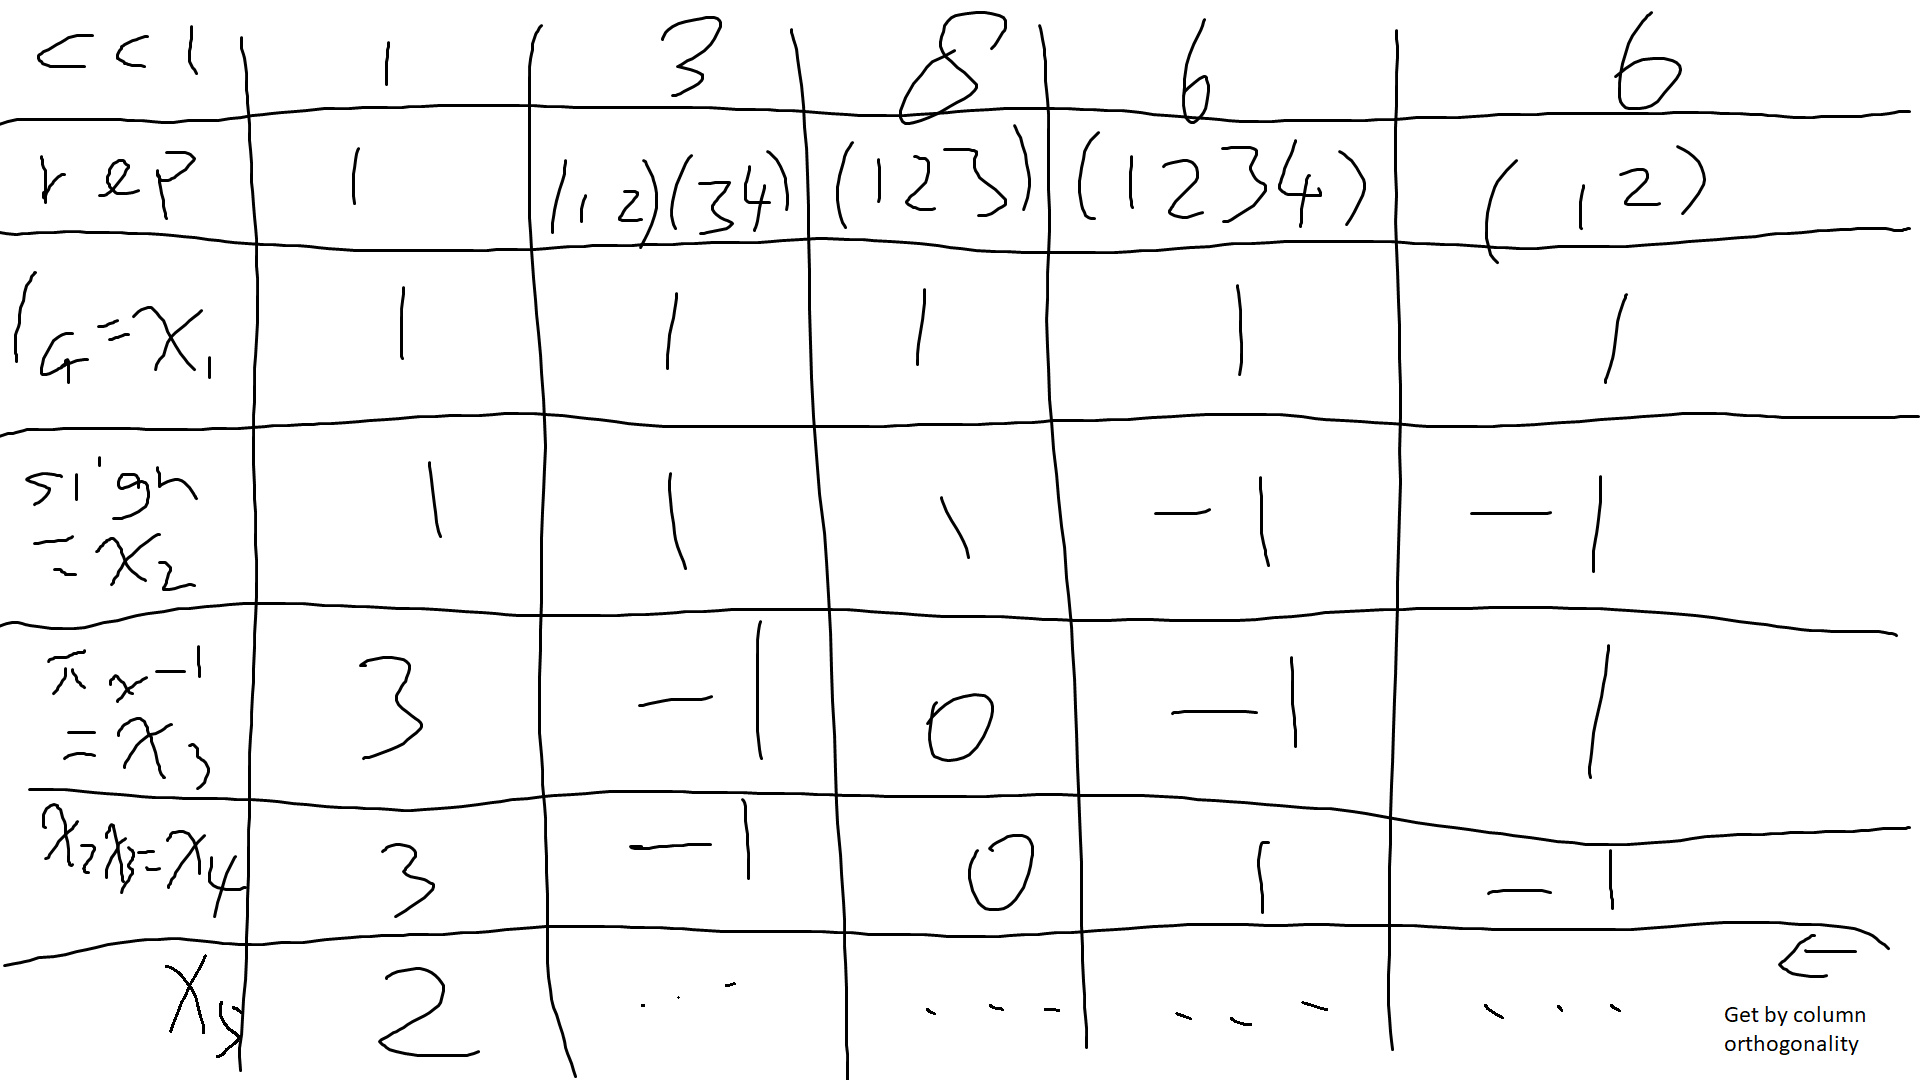
\includegraphics[scale=0.6]{image/Rep_04.png}
\end{eg}

Last lecture we were talking about using column orthogonality to find $\chi_5$. Indeed we have 
\begin{equation*}
\begin{aligned}
\chi_{reg} = \chi_1+\chi_2+3\chi_3+3\chi_4+2\chi_5
\end{aligned}
\end{equation*}
So we can use this to find $\chi_5$. Also, $S_4 / V_4 \cong S_3$ by 'lifting' -- see next chapter.


\subsection{Alternating groups}
Suppose $g \in A_n$. In 1A we've known that $|\mathcal{C}_{S_n} (g)| = |S_n:C_{S_n}(g)|$ and $|\mathcal{C}_{A_n}(g)| = |A_n : C_{A_n}(g)|$.

These are not necessarily equal. For example, $\sigma=(123) \in A_3$, $\mathcal{A}_3 (\sigma) =\{\sigma\}$, but $\mathcal{S_3}(\sigma) = \{\sigma,\sigma^{-1}\}$.

\begin{lemma} (7.9)\\
Let $g \in A_n$. Then if $g$ commutes with some odd permutation in $S_n$ then $\mathcal{C}_{S_n} (g) = \mathcal{C}_{A_n}(g)$; otherwise $\mathcal{C}_{S_n}(g)$ splits into two ccls in $A_n$ of equal size.
\end{lemma}

For example, consider $G=A_4$, so $|G| = 12$.

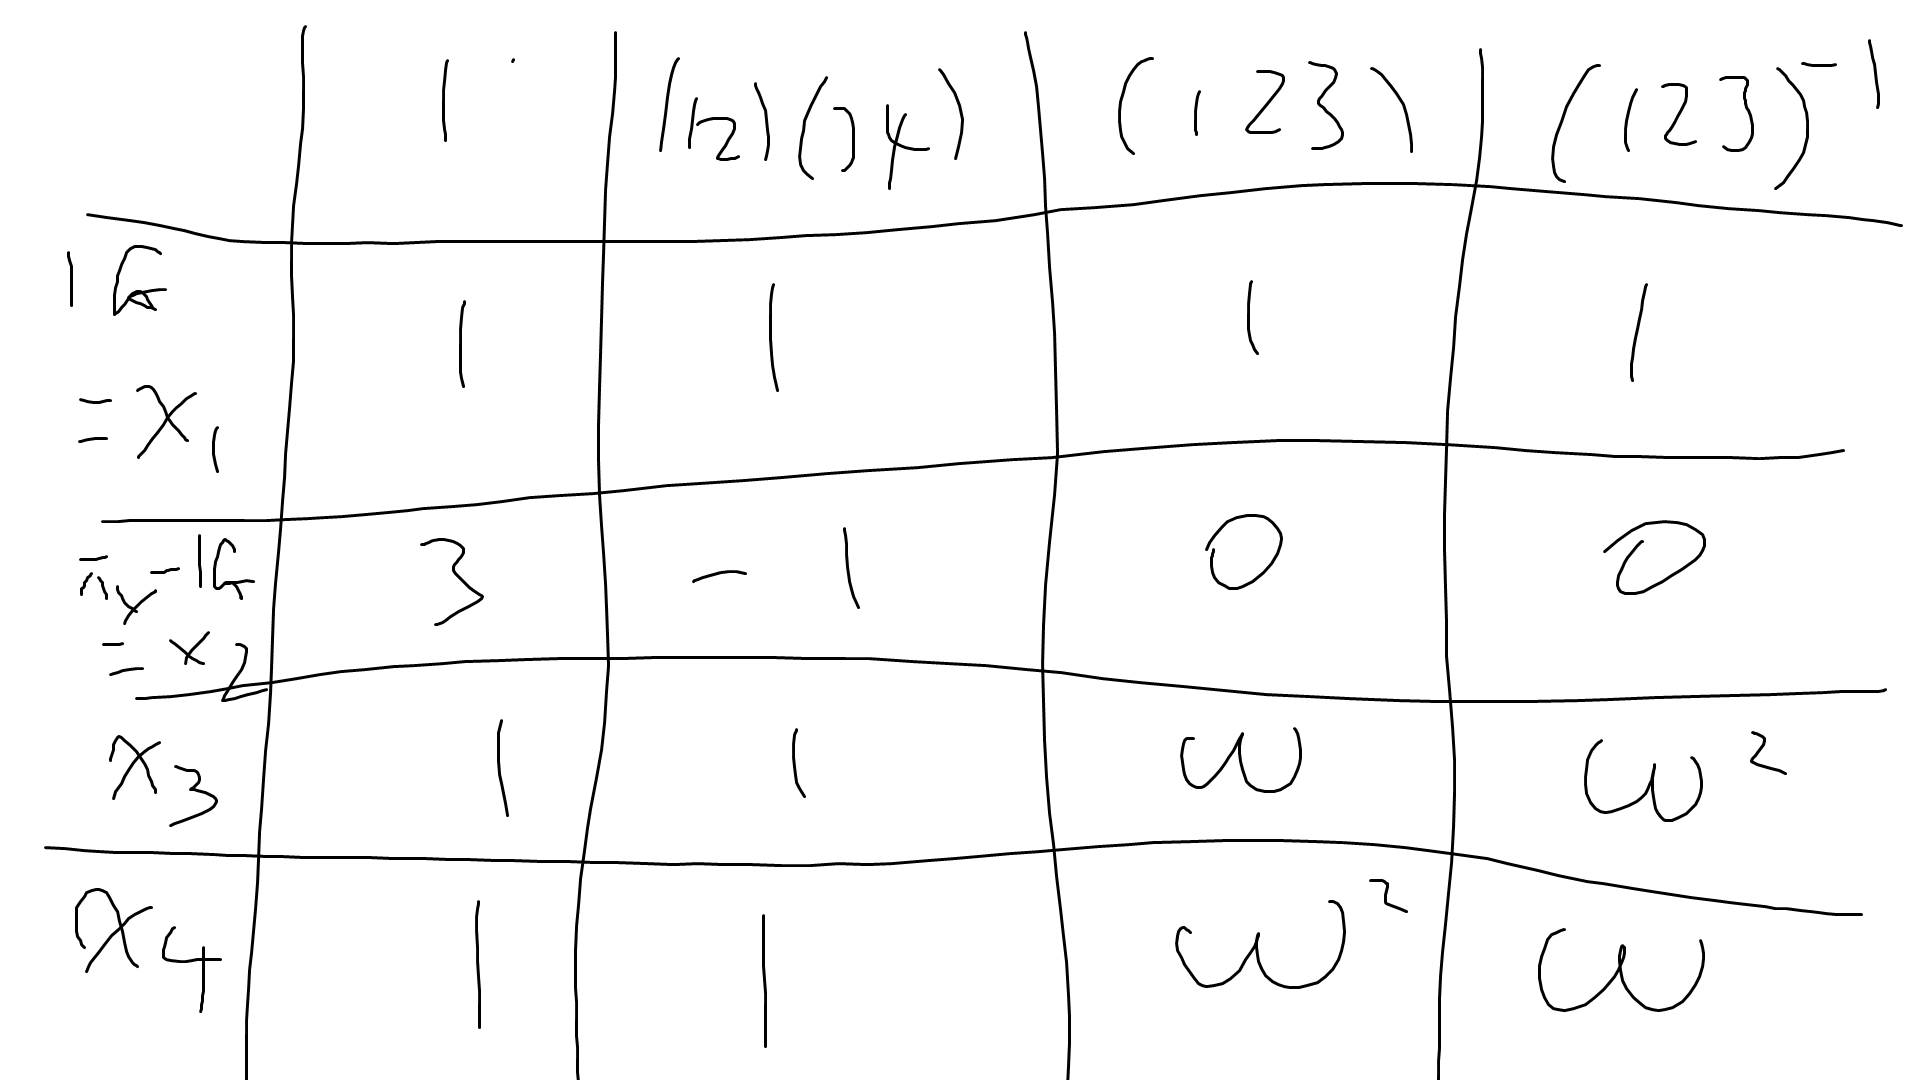
\includegraphics[scale=0.6]{image/Rep_05.png}

Note that if we ignore the second row and first column, the table becomes identical to that of $C_3 \cong G/V_4$. This is not a coincident, and is actually called \emph{lifting}.

\newpage

\section{Normal subgroups and lifting characters}
\begin{lemma} (8.1)\\
Let $N \triangleleft G$. Let $\tilde{\rho} : G/N \to GL(V)$ be a representation of $G/N$. Then
\begin{equation*}
\begin{aligned}
\rho:G &\xrightarrow{canonical} G/N &\xrightarrow{\tilde{\rho}} GL(V)\\
g & \to & \tilde{\rho}(gN)
\end{aligned}
\end{equation*}
is a representation of $G$, where $\rho(g) := \tilde{\rho}(gN)$. Moreover, $\rho$ is irreducible iff $\tilde{\rho}$ is irreducible.

The corresponding characters satisfy $\chi(g) =\tilde{\chi} (gN)$. We say that $\tilde{\chi}$ \emph{lifts} to $\chi$. The lifting $\tilde{\chi} \to \chi$ is a bijection between irreducible representations of $G/N$ and irreducible representations of $G$ with $N$ in $\ker$.

Well this looks like Q4/Q12 in the first example sheet.

\begin{proof}
Note $\chi(g) = \tr(\rho(g)) = \tr(\tilde{\rho}(gN)) = \tilde{\chi}(gN) \forall g$, and $\chi(1) = \tilde{\chi}(N)$. SO have some degree (?).

Bijection: if $\tilde{\chi}$ is a charcter of $G/N$-representaiton and $\chi$ is its lift to $G$, then $\chi(N) = \chi(1)$. Also, if $k \in N$ then 
\begin{equation*}
\begin{aligned}
\chi(k) = \tilde{\chi} (kN) = \tilde{\chi}(N) = \chi(1)
\end{aligned}
\end{equation*}
So $N \leq \ker\chi$.

Now let $\chi$ be character of $G$ with $N \leq \ker\chi$. Suppose $\rho:G \to GL(V)$ affords $\chi$. Define
\begin{equation*}
\begin{aligned}
\tilde{\rho}: & G/N &\to GL(V)\\
&gN &\to \rho(g)
\end{aligned}
\end{equation*}
Check this is well-defined (uses $N \leq \ker\chi$) and $\tilde{\rho}$ is homomorphism, hence gives representaiton of $G/N$. If $\tilde{\chi}$ is the character of $\tilde{\rho}$ then $\tilde{\chi}(gN) = \chi(g)$ $\forall g\in G$. So $\tilde{\chi}$ lifts to $\chi$.\\
Check irreducibility.
\end{proof}
\end{lemma}

\begin{lemma} (8.2)\\
The derived subgroup, $G' = \bra[a,b],a,b \in G \ket$ of $G$ is the unique minimal normal subgroup of $G$ s.t. $G/G'$ is abelian, i.e. $G/N$ is abelian $\implies G' \leq N$ and $G^{ab}=G/G'$ is abelian, where $G^{ab}$ is the \emph{abelianisation} of $G$.\\
$G$ has precisely $l=|G/G'|$ representaitons of $\dim 1$, all with kernel containing $G'$ and obtained by lifting from $G/G'$. In particular, $l | |G|$.
\begin{proof}
$G'\triangleleft G$ is an easy exercise.

Let $N \triangleleft G$. Let $h,g \in G$, so 
\begin{equation*}
\begin{aligned}
&g^{-1}h^{-1}gh \in N \iff &(gh)N = (hg)N\\
&[g,h] \iff (gN)(hN) = (hN)(gN)
\end{aligned}
\end{equation*}
So $G' \leq N \iff G/N$ is abelian. Since $G' \triangleleft G$ we deduce $G/G'$ is abelian.

By (4.5), $G/G'$ has exactly $l$ irreducible characters $\tilde{\chi}_1,...,\tilde{\chi}_l$ all of degree 1. The lifts of these to $G$ also have degree 1 and by (8.1) these are precisely the irreducible characters $\chi_i$ of $G$ s.t. $G' \leq \ker \chi_i$. But any linear character of $G$ is a homomorphism $\chi:G \to \C^*$, hence $G' \leq \ker \chi$ ($\chi(ghg^{-1}h^{-1}) = \chi(g)\chi(h)\chi(g^{-1} \chi(h)^{-1} = 1$), so the $\chi_1,...,\chi_l$ are all the linear characters of $G$.
\end{proof}
\end{lemma}

Examples:\\
(a) If $G=S_n$, show $s'_n = A_n$. Thus since $G/G' \cong C_2$, $S_n$ must have exactly two linear characters.\\
(b) Consider $G=A_4$. We've seen previously that this can be lifted from $C_3$ using (8.1),(8.2).

\begin{lemma} (8.4)\\
$G$ is not simple iff $\chi(g) = \chi(1)$ for some irreducible character $\chi \neq 1_G$ and some $1 \neq g \in G$.\\
Any normal subgroup of $G$ is the intersection of the kernels of some of the irreducible characters of $G$:
\begin{equation*}
\begin{aligned}
N =\bigcap_i \ker \chi_i
\end{aligned}
\end{equation*}
\begin{proof}
If $\chi(g) = \chi(1)$ for some non-trivial irreducible character $\chi$ (afforded by $\rho$, say). Then $g \in \ker\rho$ (5.3), so if $g \neq 1$, then $1 \neq \ker \rho \stackrel{\triangleleft}{\neq} G$.\\
If $1 \neq N \stackrel{\triangleleft}{\neq} G$, take irreducible $\tilde{\chi}$ of $G/N$, $\tilde{\chi}$ non-trivial. Lift to get an irreducible $\chi$, afforded by $\rho$ of $G$, then $N \leq \ker \rho \triangleleft G$. So $\chi(g) \ chi(1)$ for $g \in N$.\\
We claim that, if $1 \neq N \triangleleft G$, then $N$ is the intersection of the kernels of the lifts of all the irreducibles of $G/N$.\\
$\leq$ is clear from (8.1). If $g \in G \setminus N$, then $gN \neq N$. so $\tilde{\chi} (gN) \neq \tilde{\chi}(N)$ for some irreducible $\tilde{\chi}$ of $G/N$. Lifting $\tilde{\chi}$ to $\chi$, we have $\chi(g) \neq \chi(1)$.
\end{proof}
\end{lemma}
Recall $\ker \chi = \{g \in G: \chi(g) = \chi(1)\}$. (5.3) : $g \in \ker\chi \iff g \in \ker\rho$.

\newpage
\section{Dual spaces and tensor products of representations}

Recall (5.5):\\
$\bullet$ $\mathcal{C}(G)$ is $\C$-space of class functions on $G$;\\
$\bullet$ endowed with irreducible product, $\dim \mathcal{C}(G) = k$, orthonormal basis of irreducible characters of $G$ (5.6)l\\
$\bullet$ there exists an involution (ring homomorphism of order 2): $f \to f^*$ where $f^*(g) = f(g^{-1})$.

\begin{lemma} (9.1)\\
Let $\rho:G \to GL(V)$, representation over $F$, and let $V^* = Hom_F (V,F)$, dual space of $V$. Then $V^*$ is a $G$-space under 
\begin{equation*}
\begin{aligned}
(\rho^*(g)\phi)(v) = \phi(\rho(g^{-1})v)
\end{aligned}
\end{equation*}
called the \emph{dual representation} to $\rho$. Its charcater is $\chi_{\rho^*}(g) = \chi_\rho (g^{-1})$.
\begin{proof}
\begin{equation*}
\begin{aligned}
\rho^*(g_1) (\rho^*(g_2)\phi)(v) &= (\rho^*(g_2)\phi)(\rho(g_1^{-1})(v))\\
&= \phi(\rho(g_2^{-1}) \rho(g_1^{-1}) v)\\
&= \phi(\rho(g_1g_2)^{-1}(v))\\
&= (\rho^*(g_1g_2)\phi)(v)
\end{aligned}
\end{equation*}
So this is a representation. For its character, fix $g \in G$ and let $e_1,...,e_n$ be basis of $V$ of eigenvectors of $\rho(g)$, say $\rho(g) e_j = \lambda_j e_j$. Let $\varepsilon_1,...,\varepsilon_n$ be dual basis. We claim that $\rho^*(g) \varepsilon_j =\lambda^{-1}_j \varepsilon_j$:
\begin{equation*}
\begin{aligned}
(\rho^*(g)\varepsilon_j)(e_i) = \varepsilon_j(\rho(g^{-1})e_i) = \varepsilon_j\lambda_i^{-1}e_i = \lambda_j^{-1} \varepsilon_j e_i \forall i
\end{aligned}
\end{equation*}
So $\chi_{\rho^*}(g) = \sum \lambda_j^{-1}  = \chi_\rho(g^{-1})$.
\end{proof}
\end{lemma}

\begin{defi} (9.2)\\
$\rho:G \to GL(V)$ is \emph{self-dual} if $V \cong V^*$ (as $G$-spaces). Over $\C$, this holds iff $\chi_\rho(g) = \chi_\rho(g^{-1})$ ($=\overline{\chi_\rho(g)}$) $\forall g$, iff $\chi_\rho(g) \in \R$ for all $g$.
\end{defi}

Exercise: all irreducible representaitons of $S_n$ are self-dual (the ccls are determined by cycle type, so $g,g^{-1}$ are always $S_n$-conjugate. Not always true for $A_n$.

\subsection{tensor products}
Let $V,W$ be $F-$spaces, $\dim V = m$, $\dim W = n$. Fix bases $v_1,...,v_m$ and $w_1,...,w_n$ of $V,W$ respectively. The \emph{tensor product space} $V \otimes_F W$ is an $nm$-dimensional $F$-space with basis $\{v_i \otimes w_j: 1 \leq i \leq m, 1 \leq j \leq n\}$. Thus\\
(a) $V \otimes W = \{\sum_{i,j} \lambda_{ij} v_i \otimes w_j: \lambda_{ij} \in F\}$ with 'obvious' addition and scalar multiplication;\\
(b) If $v = \sum_{i} \alpha_iv_i \in V$, $w = \sum_j \beta_j w_j \in W$, define $v\otimes w:=\sum_{i,j} \alpha_i\beta_j (v_i\otimes w_j)$.

\begin{rem}
Not all elements of $V \otimes W$ are of this form: some are combinations, e.g. $v_1 \otimes w_1 + v_2 \times w-2$, which can't be further simplified. (like entangled)
\end{rem}

\begin{lemma} (9.3)\\
(i) For $v \in V$, $w \in W$, $\lambda \in F$, $(\lambda v) \otimes w = \lambda (v\otimes w) = v \otimes (\lambda w)$;\\
(i) If $x_1,x_2,x \in V$, $y_1,y_2,y \in W$, then 
\begin{equation*}
\begin{aligned}
(x_1+x_2) \otimes y = (x_1 \otimes y) + (x_2 \otimes y),\\
x \otimes (y_1+y_2) = (x \otimes y_1) + (x \otimes y_2)
\end{aligned}
\end{equation*}
\begin{proof}
(i) $v = \sum \alpha_i v_i$, $w = \sum \beta_j w_j$. Then just multiply out everything we get the desired equality. (ii) is similar.
\end{proof}
\end{lemma}

\begin{lemma} (9.4)\\
If $\{e_1,...,e_m\}$ is a basis of $V$, $\{f_1,...,f_n\}$ is a basis of $W$, then $\{e_i \otimes f_j: 1 \leq i \leq m,1 \leq j \leq n\}$ is a basis of $V \otimes W$.
\begin{proof}
Writing $v_k = \sum_i \alpha_{ik} e_i$, $w_l = \sum_j \beta_{jl} f_j$, we have
\begin{equation*}
\begin{aligned}
v_k \otimes w_l = \sum \alpha_{ik} \beta_{jl} e_i \otimes f_j
\end{aligned}
\end{equation*}
Hence $\{e_i \otimes f_j\}$ spans $V \otimes W$ and, since we have $nm$ of them, they form a basis.
\end{proof}
\end{lemma}

\begin{rem}
One can define $V \otimes W$ in a basis-independent way in the first place, see Teleman chapter 6.
\end{rem}

\begin{prop} (9.5)\\
Let $\rho: G \to GL(V)$, $\rho': G \to GL(V')$ be representations of $G$. Define $\rho \otimes \rho': G \to GL(V \otimes V')$ by
\begin{equation*}
\begin{aligned}
(\rho \otimes \rho') (g) : \sum \lambda_{ij} v_i \otimes w_j \to \sum \lambda_{ij} \rho(g) v_i \otimes \rho'(g) w_j
\end{aligned}
\end{equation*}
Then $\rho \otimes \rho'$ is a representation of $G$ with character
\begin{equation*}
\begin{aligned}
\chi_{\rho \otimes \rho'} (g) = \chi_\rho(g) \chi_{\rho'} (g) \forall g \in G
\end{aligned}
\end{equation*}
Hence product of two characters of $G$ is still a character of $G$.
\begin{proof}
On Tuesday.
\end{proof}
\end{prop}

(After lecture 11: this is the first notes to get beyond 1000 lines!)

\begin{rem} (9.6)\\
Sheet 1, Q2 says $\rho$ irreducible, $\rho'$ of degree 1, then $\rho \otimes \rho'$ irreducible; if $\rho'$ is not of $\deg$ 1 this is usually false.
\end{rem}

\begin{proof} (of 9.5)\\
It's clear that $(\rho \otimes \rho') (g) \in GL(V \otimes V')$ $\forall g \in G$ and so $\rho \otimes \rho'$ is a homomorphism $G \to GL(V \otimes V')$. Let $g \in G$. Let $V_1,...,v_m$ be basis of $V$ of eigenvectors of $\rho(g)$; let $w_1,...,w_n$ be a basis of $V'$. Say: 
\begin{equation*}
\begin{aligned}
\rho(g) v_j = \lambda_j v_j, \rho'(g) w_j = \mu_j w_j
\end{aligned}
\end{equation*}
Then 
\begin{equation*}
\begin{aligned}
(\rho \otimes \rho') (g) (v_i \otimes w_j) &= \rho(g) v_i \otimes \rho'(g) w_j\\
&= \lambda_i v_i \otimes \mu_j w_j\\
&= (\lambda_i \mu_j) (v_i \otimes w_j)
\end{aligned}
\end{equation*}
So $\chi_{\rho \otimes \rho'}(g) = \sum_{i,j} \lambda_i \mu_j = (\sum \lambda_i)(\sum\lambda_j) = \chi_\rho(g)\chi_{\rho'}(g)$
\end{proof}

Now work over $\C$. Take $V=V'$ and define $V^{\otimes 2} = V \otimes V$.\\
Let
\begin{equation*}
\begin{aligned}
\tau: \sum \lambda_{ij} v_i \otimes v_j \to \sum \lambda_{ij} \lambda_j \otimes v_i
\end{aligned}
\end{equation*}
which is a linear $G$-endomorphism of $V^{\otimes 2}$, s.t. $\tau^2 =1$ (so eigenvalues $\pm 1$).

\begin{defi} (9.7)\\
\begin{equation*}
\begin{aligned}
S^2 V = \{v \in V^{\otimes 2}: \tau(x) = x\},\\
\wedge^2 V = \{x \in V^{\otimes 2}: \tau(x) = -x\}
\end{aligned}
\end{equation*}
known as the \emph{symmetric square} of $V$ and \emph{exterior square} of $V$ respectively.
\end{defi}

\begin{lemma} (9.8)\\
$S^2 V$ and $\wedge^2 V$ are $G$-subspaces of $V^{\otimes 2}$ and $V^{\otimes 2} \cong S^2 V \otimes \wedge^2 V$. $S^2 V$ has basis $\{v_iv_j := v_i \otimes v_j + v_j \otimes v_i: 1 \leq i \leq j \leq n\}$, and $\wedge^2 V$ has basis $\{v_i \wedge v_j:=v_i \otimes v_j - v_j \otimes v_i: 1 \leq i < j \leq n\}$. Hence we have $\dim S^2 V = \frac{1}{2}n(n+1)$ and $\dim \wedge^2 V = \frac{1}{2} n(n-1)$.
\begin{proof}
Exercise in linear algebra.\\
To show $V^{\otimes 2}$ is reducible, write $x \in V^{\otimes 2}$ as $x=\frac{1}{2} (x+\tau(x)) + \frac{1}{2} (x-\tau(x))$, which is in $S^2 V$ and $\wedge^2 V$ respectively.
\end{proof}
\end{lemma}

In fact, $V^{\otimes 2}$, $V^{\otimes 3} = V \otimes V \otimes V$, ...,etc. are never irreducible if $\dim V > 1$.

\begin{lemma} (9.9)\\
If $\rho:G \to GL(V)$ is a representation affording character $\chi$, then $\chi^2 = \chi_S + \chi_\wedge$ where $\chi_s$ ($=S^2 \chi$) is the character of $G$ in the subrepresentation $S^2 V$, and $\chi_\wedge$ ($=\wedge^2 \chi)$ is the character of $G$ in the subrepresentation $\wedge^2 V$. Moreover, for $g \in G$,
\begin{equation*}
\begin{aligned}
\chi_s(g) = \frac{1}{2} (chi^2(g) + \chi(g^2)),
\chi_\wedge(g) = \frac{1}{2} (\chi^2(g) - \chi(g^2)).
\end{aligned}
\end{equation*}
\begin{proof}
Let's compute the characters $\chi_s,\chi_\wedge$. Fix $g \in G$. Let $v_1,...,v_n$ be a basis of eigenvectors of $\rho(g)$, say $\rho(g)v_i = \lambda_i v_i$ (we drop the $\rho$ to write $g v_i = \lambda_i v_i$ for simplicity below). Then
\begin{equation*}
\begin{aligned}
g v_i v_j = \lambda_i \lambda_j v_i v_j\\
g v_i \wedge v_j = \lambda_i \lambda_j v_i \wedge v_j
\end{aligned}
\end{equation*}
Hence $\chi_s(g) = \sum_{1 \leq i \leq j \leq n} \lambda_i\lambda_j$ and $\chi_\wedge(g) = \sum_{1 \leq i < j \leq n} \lambda_i \lambda_j$. Now,
\begin{equation*}
\begin{aligned}
(\chi(g))^2 &= (\sum \lambda_i)^2\\
&= \sum \lambda_i^2 + 2\sum_{i < j} \lambda_i \lambda_j\\
&= \chi(g^2) + 2\sum_{i < j} \lambda_i \lambda_j\\
&= \chi(g^2) + 2 \chi_\wedge (g)
\end{aligned}
\end{equation*}
So $\chi_\wedge (g) = \frac{1}{2} (\chi^2 (g) - \chi(g^2))$. But $\chi^2 = \chi_s + \chi_\wedge$ so we get the expression for $\chi_s(g)$.
\end{proof}
\end{lemma}

\begin{eg} (9.10)\\
Consider our usual example $G=S_4$ (see 7.8).

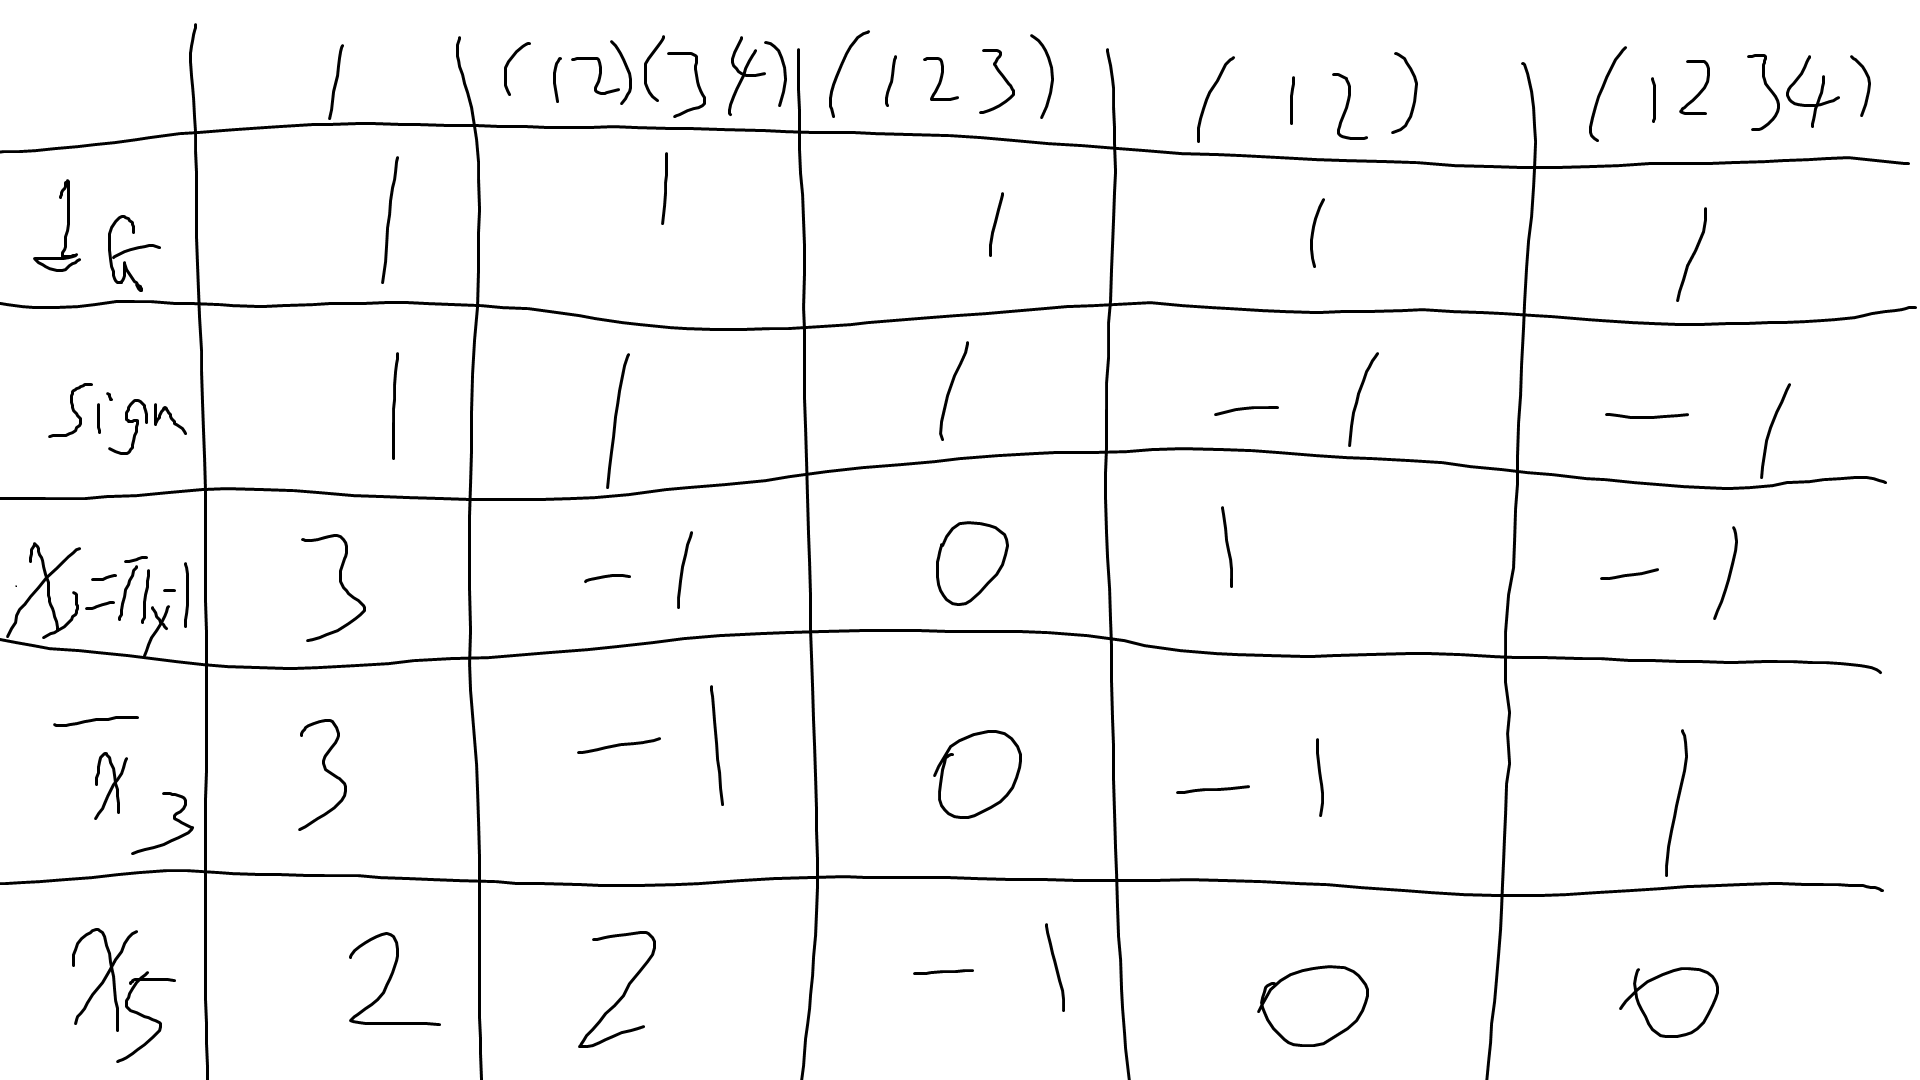
\includegraphics[scale=0.5]{image/Rep_06.png}

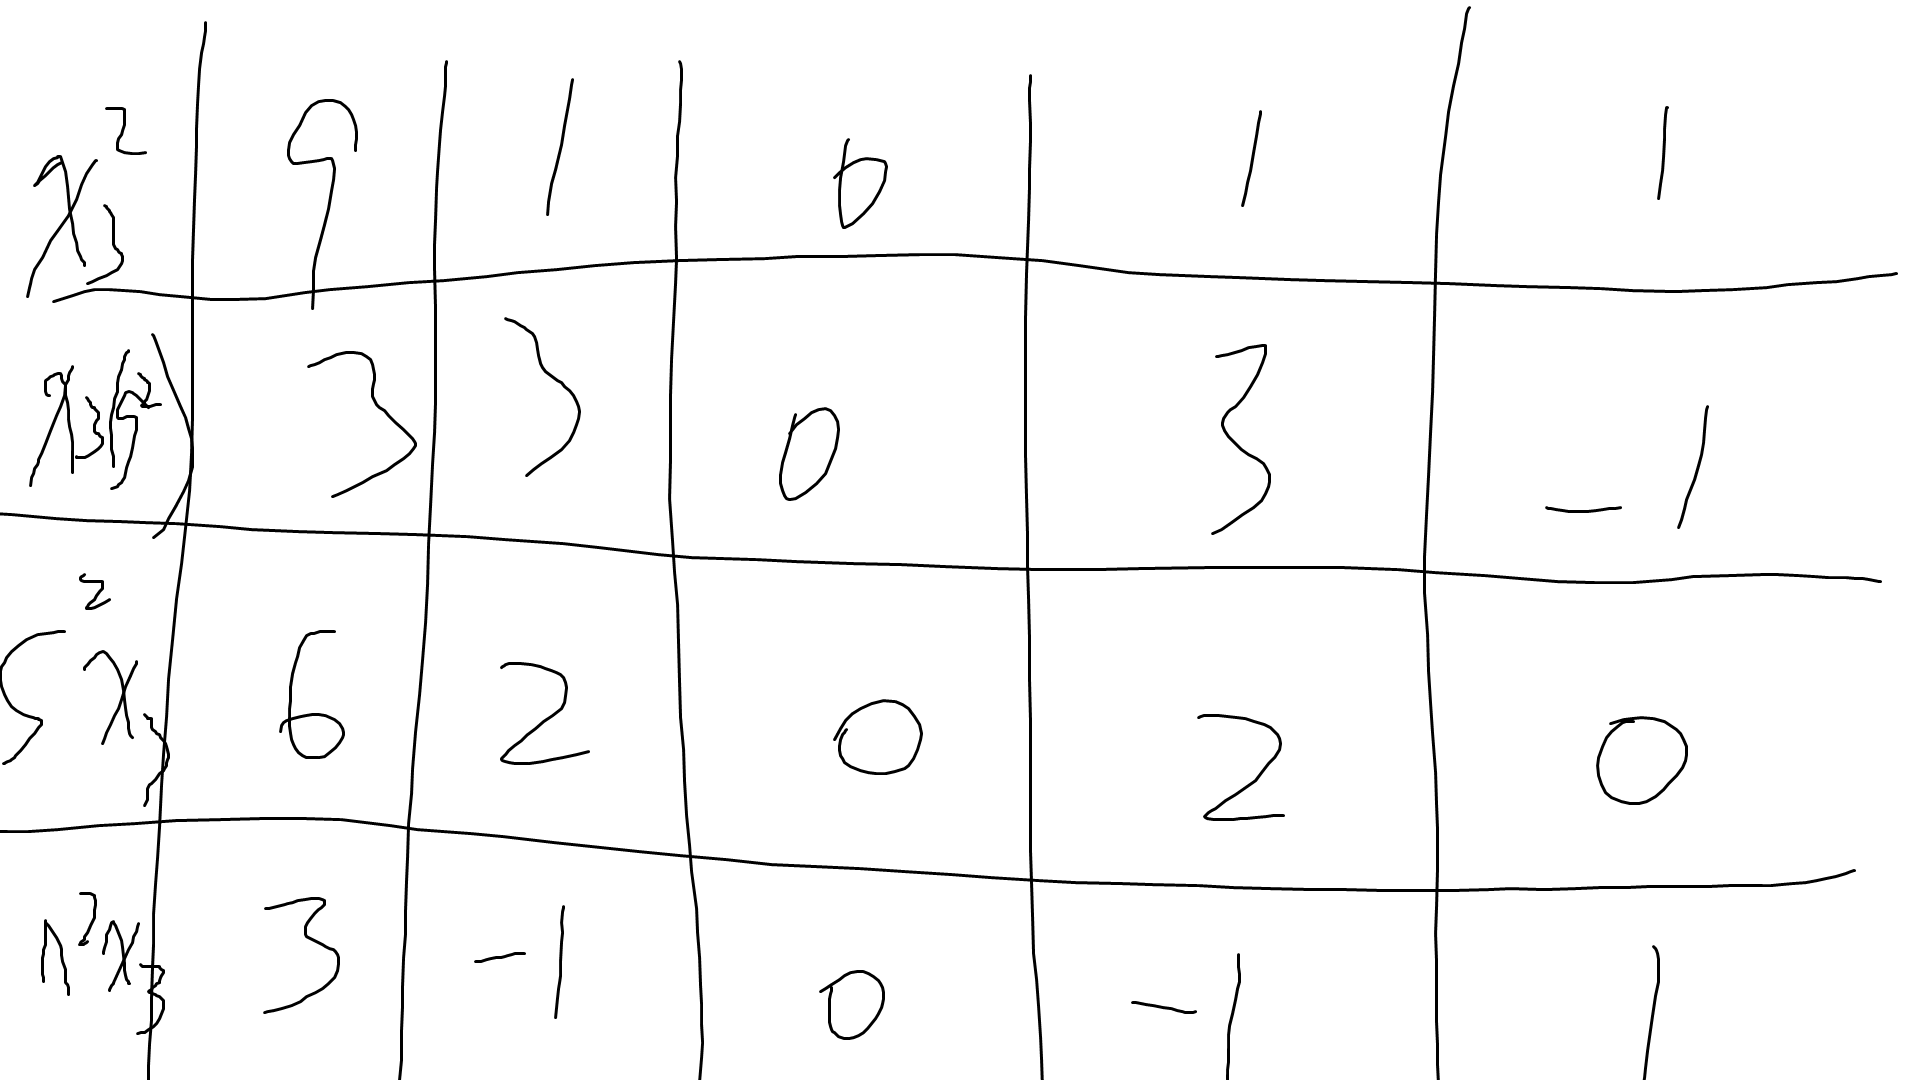
\includegraphics[scale=0.5]{image/Rep_07.png}

Notice that $\wedge^2 \chi_3 = \bar{\chi}_3$ (irreducible since $\bra \chi_\wedge,\chi_\wedge\ket = 1$),\\
$S^2 \chi_3 = 1+\chi_3+\chi5$: The inner product is 3 and it contains $1$ ,$\chi_3$, so the one left is $\chi_5$.
\end{eg}

Characters of $G \times H$ (seen in (4.5) for abelian groups):\\
\begin{prop} (9.11)\\
If $G,H$ are finite groups with irreducible characters $\chi_1,...,\chi_k$ and $\psi_1,...,\psi_r$ respectively, then the irreducible characters of the direct product $G \times H$ are precisely $\{\chi_i \psi_j:1 \leq i \leq k, 1 \leq j \leq r\}$, where $\chi_i \psi_j (g,h) = \chi_i*g( \psi_j(h)$.
\begin{proof}
If $\rho:G \to GL(V)$, $\rho':H \to GL(W)$ affording $\chi$ and $\psi$ respectively, then
\begin{equation*}
\begin{aligned}
\rho \otimes \rho': &G \times H \to &GL(V \otimes W)\\
&(g,h) \to &\rho(g) \otimes \rho'(h)
& &v_i \otimes w_j \to \rho(g) v_i \otimes \rho'(h) w_j
\end{aligned}
\end{equation*}
is a representation of $G \times H$ on $V \otimes W$ by (9.5), and $\chi_{\rho \otimes \rho'} = \chi\psi$, again by (9.5).\\
We claim that $\chi_i \psi_j$ are distinct and irreducible:
\begin{equation*}
\begin{aligned}
\bra \chi_i \psi_j,\chi_r\psi_s \ket_{G \times H} &= \frac{1}{|G \times H|} \sum_{(g,h)} \overline{\chi_i\psi_j (g,h)} \chi_r \psi_s (g,h)\\
&= (\frac{1}{|G|} \overline{\chi_i(g)} \chi_r(g)) (\frac{1}{|H|} \sum_h \overline{\psi_j(h)} \psi_s(h))\\
&= \delta_{ir} \delta_{js}
\end{aligned}
\end{equation*}
...tbc.\\
Let's complete on $\chi_i\psi_j$ being distinct and irreducible:\\
Complete set: $\sum_{i,j} (\chi_i\psi_j)(1)^2 = \sum_i \chi_i(1)^2 \sum_j \psi_j(1)^2 = |G| |H| = |G \times H|$
\end{proof}
\end{prop}

\subsection{Symmetric and extreior powers}
Let $V$ be a vector space, $\dim_F V = d$, with basis $\{v_1,...,v_d\}$. Let $V^{\otimes n} = V \otimes ... \otimes V$, with basis $\{v_{i_1} \otimes ... \otimes v_{i_n} : (i_1,...,i_n) \in \{1,...,d\}^n\}$, so $\dim V^{\otimes n} = d^n$.

$S_n$-action: for any $\sigma \in S_n$, we can define linear map
\begin{equation*}
\begin{aligned}
\sigma: &V^{\otimes n} \to &V^{\otimes n}\\
v_1 \otimes ... \otimes v_n \to &v_{\sigma^{-1}(1)} \otimes ... \otimes v_{\sigma^{-1}(n)}
\end{aligned}
\end{equation*}
for $v_1,...,v_n \in V$, permuting posutums of vectors in a tensor.

For example, $(12)(v_1\otimes v_2 \otimes v_3) = v_2 \otimes v_1 \otimes v_3$, $(13)(v_2 \otimes v_1 \otimes v_3) = v_3 \otimes v_1 \otimes v_2$.

Check that this defines a representation of $S_n$ on $V^{\otimes n}$ (extended linearly).

$G$-action: given representation $\rho:G \to GL(V)$, then the action of $G$ on $V^{\otimes n}$ is
\begin{equation*}
\begin{aligned}
\rho^{\otimes n} (g) : v_1 \otimes ... \otimes v_n = \rho(g) v_1 \otimes ... \otimes \rho(g) v_n
\end{aligned}
\end{equation*}
extended linearly, and this commutes with the $S_n$-action. We can decompose $V^{\otimes n}$ as $S_n$-module, and each isotypical component (4.?) is $G$-invariant subspace of $V^{\otimes n}$. In particular:

\begin{defi} (9.12)\\
For $G$-space $V$, define\\
(i) the $n$th symmetric power of $V$, $S^n V = \{x \in V^{\otimes n}: \sigma(x) = x \forall \sigma \in S_n\}$;\\
(ii) the $n$th exterior power of $V$, $\wedge^n V = \{x \in V^{\otimes n}: \sigma(x) = sign(\sigma)x \forall \sigma \in S_n\}$.\\
Both are $G$-subspaces of $V^{\otimes n}$, but for $n>2$, $S^n V \oplus \wedge^n V \lneq V^{\otimes n}$, so in general there are lots of others for the $S_n$-action.
\end{defi}

(9.13) See Sheet 3 Q7 for bases of $S^n V$, $\wedge^n V$ and their characters.

\subsection{Tensor algebra}
Take $char F = 0$.

\begin{defi} (9.14)\\
Let $T^n V = V^{\otimes n}$. The tensor algebra of $V$ is $TV := \oplus_{n \geq 0} T^n V$, $T^0 V = F$.\\
This is $F$-space and is a (non-commutative) graded ring with product $x \in T^n V$, $y \in T^m V$ , $x \cdot y = x \otimes y \in T^{n+m} V$.\\
There are two graded quotient rings
\begin{equation*}
\begin{aligned}
SV = TV /(\text{ideal generated by all } U \otimes V - V \otimes U)\\
\wedge V = TV / \text{ ideal generated by all }V \otimes V
\end{aligned}
\end{equation*}
called the symmetric algebra and exterior algebra respectively.
\end{defi}

\begin{defi} (9.15)\\
The $2$-submodule of $\mathcal{C}(G)$ spanned by irreducible characters of $G$ is the character ring of $G$, $R(G)$. Elements of $R(G)$ are called generalised/virtual characters if $\psi = \sum n_\chi \chi$, $n_\chi \in \Z$ correspondingly.\\
$\bullet$ $R(G)$ is a commutative ring and any generalised character is a difference of two characters, $\psi = \alpha - \beta$:\\
$\alpha = \sum_{n_\chi \geq 0} n_\chi \chi, \beta = -\sum_{n_\chi < 0} n_\chi \chi$.\\
The $\{\chi_i\}$ form a $\Z$-basis for $R(G)$ as a free $\Z$-module.\\
$\bullet$ Suppose $\psi$ is virtual character and $\bra\psi,\psi\ket = 1$ and $\psi(1) > 0$. Then $\psi$ is actually the character of an irreducible representation of $G$.\\
List irreducible characters of $G$: $\chi_1,...,\chi_k$, $\psi = \sum n_i \chi_i$; orthonormality says $\bra\psi,\psi\ket = \sum n_i^2$, so $\sum n_i^2 = 1$, meaning $n_i = \pm 1$ for exactly one $i$ and $n_j = 0$ for $j \neq i$. Since $\psi(1)>0$, we must have $n_i = +1$.\\
$\bullet$ Henceforth we don't distinguish between a character and its negative and we often study generalised characters of norm 1 rather than irreducible characters.
\end{defi}

\newpage
\section{Restriction and induction}
Throughout we set $H \leq G$, $F = \C$.

\begin{defi} (10.1, restriction)\\
Let $\rho:G \to GL(V)$ be representation affording $\chi$. We can think of $V$ as a $H$-space by restricting attention to $h \in H$. We then get
\begin{equation*}
\begin{aligned}
Res_H^G \rho : &H \to &GL(V)
\end{aligned}
\end{equation*}
This is sometimes written as $\rho_H$ or $\rho\downarrow_H$, the restriction of $\rho$ to $H$. It affords the character $Res_H^G \chi = \chi_H = \chi \downarrow_H$.
\end{defi}

\begin{lemma} (10.2)\\
If $\psi$ is any non-zero character of $H \leq G$, then there exists irreducible charcater $\chi$ of $G$ s.t. $\bra Res_H^G \chi, \psi \ket_H \neq 0$. We say $\psi$ is a constituent of $Res_H^G \chi$.
\begin{proof}
\begin{equation*}
\begin{aligned}
0 \neq \frac{|G|}{|H|} \psi(1) = \bra \pi_{reg} \downarrow_H ,\psi\ket = \sum_1^k \deg \chi_i \bra \chi_i \downarrow_H ,\psi\ket
\end{aligned}
\end{equation*}
where $\psi_i$ are irreducible characters of $G$.
\end{proof}
\end{lemma}

\iffalse
\begin{equation*}
\begin{aligned}

\end{aligned}
\end{equation*}
\fi

\end{document}
